%\chapter{Microbial Community Analysis: Metagenomics and Metatranscriptomics}
%\label{chapter:B}

\section{Abstract}

Methane is one of the most potent and common greenhouse gases.
In nature, specialized bacteria called methanotrophs are able to consume methane as their only carbon and energy source \cite{murrell2009}.
Deeper understanding of these microbes sheds light on a significant natural green house gas remediation system.
The sediment of Lake Washington has served as a model ecosystem for methanotrophy studies \cite{auman2002, kalyuzhnaya2004, costello2002, kalyuzhnaya2011isolates, mctaggart2015, kalyuzhnaya2015} for decades.
Recent advances in high-throughput sequencing technology provided opportunities to observe the complex communities supported by methanotrophic methane oxidation in a more natural state than has been possible previously.
This study analyzes serial propagations of Lake Washington sediment incubated with methane as the only carbon and energy source, from both a metagenomics and metatranscriptomics perspective.
Inference of which microbes dominate the samples, and what metabolic functions are active are discovered.
The importance of \ce{O_2} as a factor in community composition and function is highlighted.

\section{Introduction}
\subsection{Lake Washington Methane Cycling Studies}

%The Lidstrom Lab has studied methanotrophic oxidation of methane in Lake Washington sediment for decades.
Methanotrophs are concentrated at the transition from aerobic to anaerobic soil in lake sediments.
This interface corresponds to both availability of methane, which rises from below, and \ce{O_2} from above \cite{lidstrom1984gradients, kuivilal1988, auman2000gradients}. %, which is required because methane is more reduced than biomass.
This microenvironment is rich in methanotrophs, methylothrophs, and other species.
When natural sediment samples are incubated in the lab with methane as the only food source, a high abundance of non-methanotrophs is often supported \cite{oshkin2015LW}.
Many of the abundant non-methanotrophs are methylotrophs, presumably consuming methanol, an intermediate of methane metabolism.
There are also many species which can only grow using multi-carbon compounds, and therefore must be consuming excreted organic multi-carbon compounds, or cell biomass.
Trends in the types of communities that form in these sediment incubations have been observed  \cite{oshkin2015LW}.
Some species pairs appear to occur more than others.
%Understanding the metabolic diversity of methanotrophs and methylotrophs in the sediment will advance understanding of why certain partnerships tend to occur, as well as understanding of a significant natural greenhouse gas mitigation system.

%Isolates first, but now new tools
% good resource: Methylotrophy in a Lake: from Metagenomics to Single-Organism Physiology https://www-ncbi-nlm-nih-gov.offcampus.lib.washington.edu/pmc/articles/PMC3147377/#B20
Early studies addressed these questions by sampling specific types of DNA from Lake Washington sediment (e.g. \cite{auman2002, costello2002, nercessian2005}), and studying isolates for which genome sequences were not available \cite{auman2000gradients, kalyuzhnaya2005Methylosarcina, kalyuzhnaya2006methylotenera}.
Later, significant effort was put toward isolation and sequencing of more species known to thrive in Lake Washington
    \cite{kalyuzhnaya2011isolates, beck2015isolates, mctaggart2015, kalyuzhnaya2015} to better understand these communities.
%These single species' metabolism can be further studied with transcriptomics and other tools (e.g. Chapter \ref{chapter:A}).
% (doesn't fit!) These strains can also be used as reference DNA for aligning shotgun sequencing reads.
%Furthermore, mixtures of small number of these pre-defined strains can be used to probe the potential of different partnerships and the underlying biology \cite{yu2016synthetic}.

% meta
Awareness that not all microbes can be isolated \cite{kaeberlein2002, stewart2012}, and that microbes probably behave differently when growing in communities due to influence of other microbes \cite{yu2016synthetic} motivates study of these microbes in their natural community compositions.
The omics studies used to observe pure cultures (e.g. Chapter \ref{chapter:A}) can be applied to communities, though analysis becomes much more challenging.
When omics methods are applied to mixed populations of organisms, the prefix "meta" is applied, resulting in terms such as  "metatranscriptomics".
Correspondingly the term "metagenomics" is used to describe sequencing the DNA of the community to allow inference of the abundant taxa and their genetic composition.
Having the paired metagenomic and metatranscriptomic data allows estimation of gene expression for those microbes, by mapping sequences to the reference DNA identified from the metagenomes.

Previous metagenomics and metatranscriptomics studies of Lake Washington sediment have highlighted dominance of the methanotrophic family \textit{Methylococcaceae} \cite{beck2013LW, beck2014LW, oshkin2015LW, hernandez2015LW} (Figure \ref{fig:taxonomy}).
These methanotrophs provide substrates for non-methanotrophic methylotrophs to grow \cite{beck2013LW}.
The particular methanotroph species and methylotroph species that dominate the sample are known to be influenced by \ce{O_2} availability \cite{hernandez2015LW}.
In previous studies, it was noted that low \ce{O2} tensions select for \mbox{\textit{Methylotenera/Methylobacter}} partnerships whereas high \ce{O2} tensions select for  \mbox{\textit{Methylophilus/Methylosarcina}} partnerships \cite{hernandez2015LW}.
There is also a revolving cast of (mostly) non-methylotrops including Burkholderiales and Bacteroidetes \cite{kalyuzhnaya2008Burkholderiales, beck2014LW}.  % Burkholderiales is an order (not italics).  Bacteroidetes is a Phylum.
Better understanding of the metabolic roles that each of these species play, and why certain partnerships tend to form would provide insight into this greenhouse-gas mitigating microbial community.

\begin{figure}[H]
\centering
    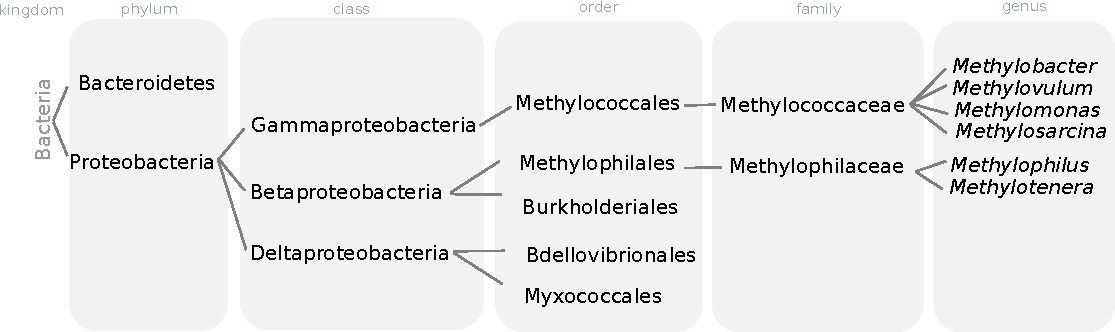
\includegraphics[width=1.0\textwidth]{./tex/chapter2/figures/170311_taxonomy_overview.pdf}
    \begin{singlespace}
    \caption[Taxonomy of microbes known to factor into methane oxidation in Lake Washington sediment]{
       Taxonomy of microbes that often appear in methane incubations of Lake Washington sediment.
       The family \textit{Methylococcaceae} is methanotrophic.
       The family \textit{Methylophilaceae} includes non-methanotrophic methylotrophs.
       Burkholderiales grow on multi-carbon compounds, but in addition, some are methylotrophs.}
    \label{fig:taxonomy}
    \end{singlespace}
\end{figure}

\subsubsection{Goals of this study}
This study aims to identify the major methanotrophic, methylotrophic, and other microbial species that together enable methane consumption in Lake Washington, as well as to deduce the contribution of each taxa to the community metabolism.
Identification of which methanotrophs dominate in natural communities provides insights into how good past isolate studies reflect the true drivers of methane oxidation.
Identification of which metabolic pathways are expressed by these methanotrophs and the accompanying non-methanotrophs informs the mechanism of methane oxidation in this natural system.
Understanding the contribution of each microbe to the community metabolism allows hypotheses about genetic factors in methanotroph/methylotroph partnerships.

%For example, this study also aims to address the relative importance of two functionally redundant methanol dehydrogenase enzymes: Xox-MDH and Mxa-MDH. (cite).
%TODO: write more about this if I get results in the area.
%TODO: Some methylotrophs only have Xox.  So they are using it, or absent.

% --- How this dataset is poised to address these questions:    Experimental design: (don't make it too methodsy!)
The experimental design chosen to answer these questions is show in in Figure \ref{fig:experimental_design}.

\begin{figure}[H]
\centering
    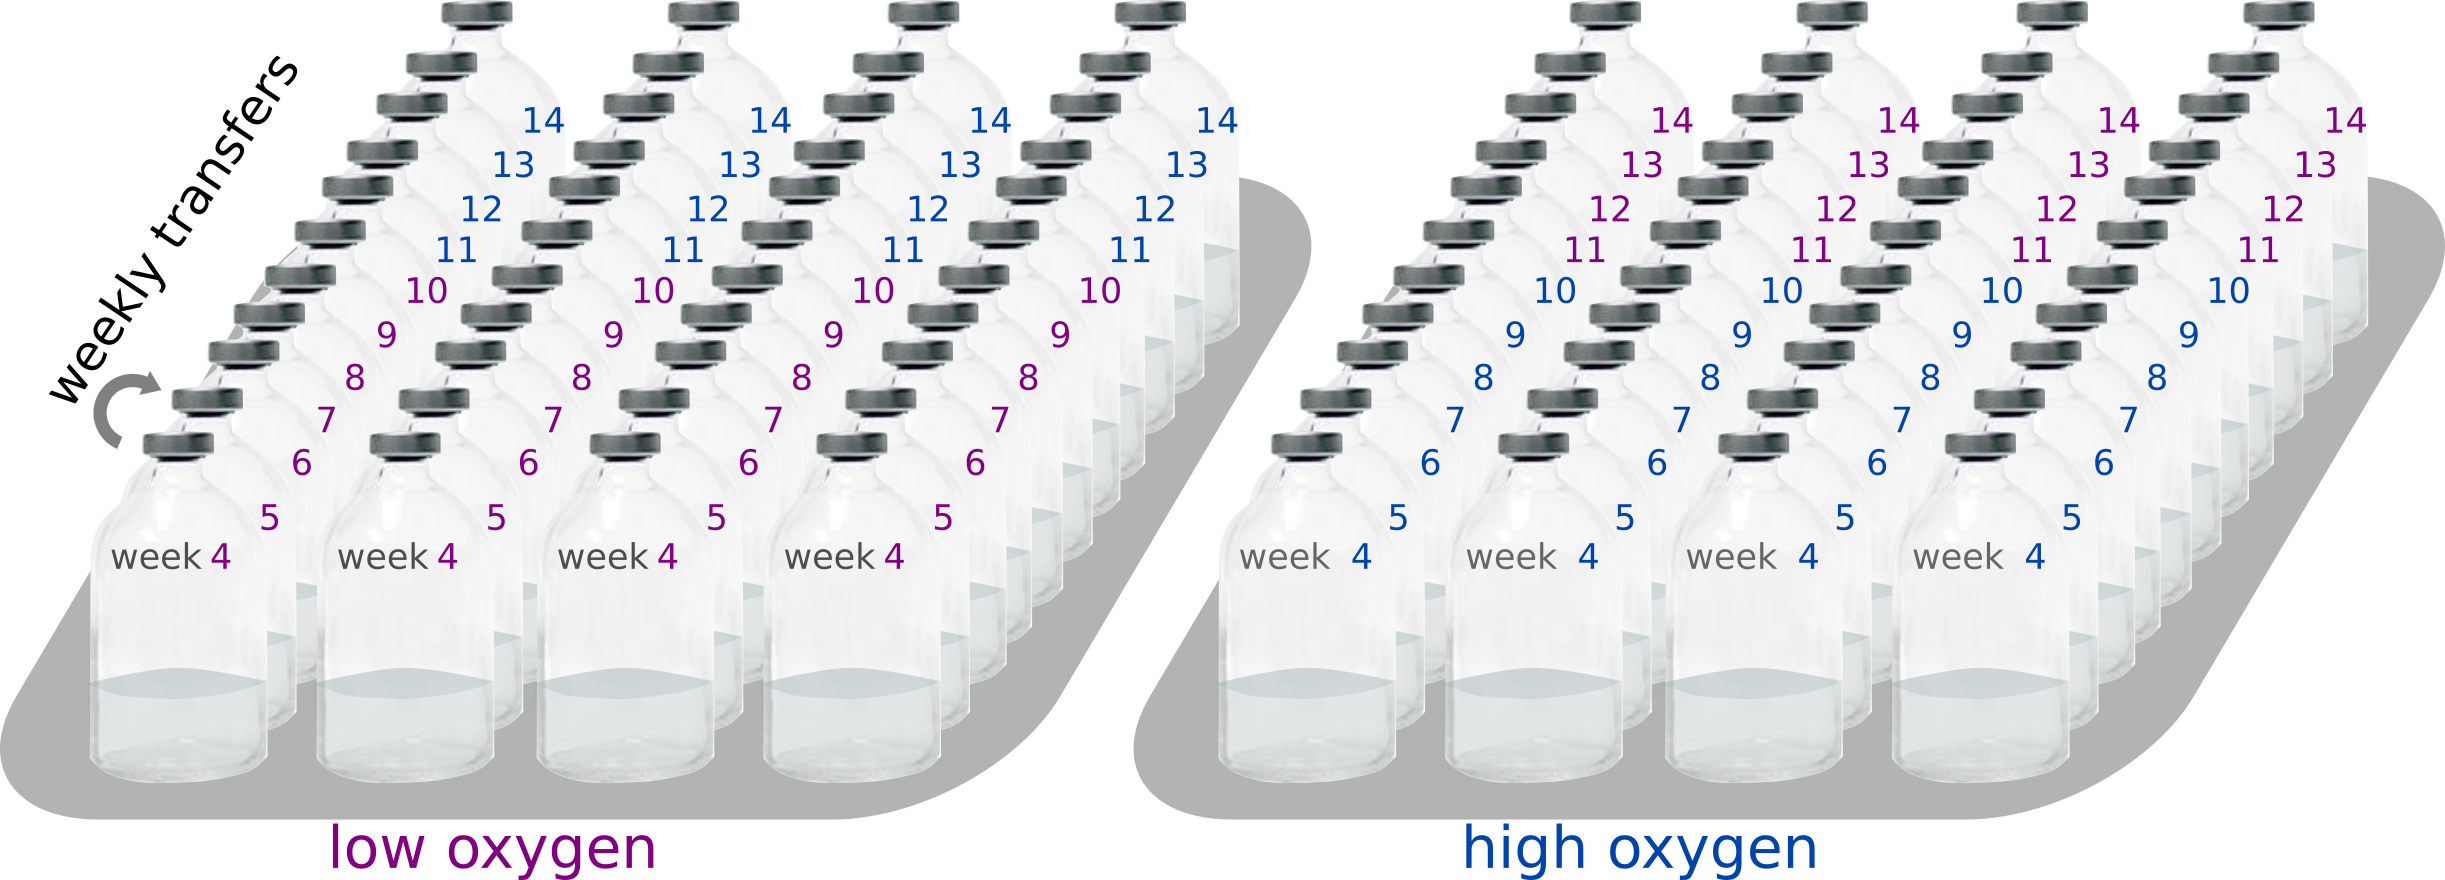
\includegraphics[width=1.0\textwidth]{./tex/chapter2/figures/170311_experimental_design_meta4--2_colors.png}
    \begin{singlespace}
    \caption[Experimental design for the data underlying Chapters \ref{chapter:A} and \ref{chapter:B}]{
	Experimental design for the data underlying Chapters \ref{chapter:A} and \ref{chapter:B}.
	Sediment from Lake Washington was thawed from -80$^o$C and cultured in 8 different bottles,
        half of which were provided with low \ce{O_2}, and half of which were provided with high \ce{O_2} (see methods).
	   Bottles were serially transferred for a total of 14 weeks.
	   The last four bottles in each series are at the opposite \ce{O_2} condition of the original experimental design
        (indicated by bottle label color switch).
	   Metagenomes and metatranscriptomes were obtained for weeks 4-14, resulting in 88 metagenomes and 88 metatranscriptomes.
	   }
    \label{fig:experimental_design}
    \end{singlespace}
\end{figure}

This relatively simple experimental design, including high degree of replication for studies of this type, was chosen to provide statistical power despite differences across replicates and measurement noise.
Variation across replicates can arise from stochasticity as communities rarefy, and are compounded by the noise-generating steps of nucleic acid extraction, ribosomal RNA removal (in the case of metatranscriptomics), library prep, and the sequencing process.
The most important environmental variable identified in previous studies, the \ce{O_2} availability, was modulated while holding all other variables constant.
Availability of sequenced isolate strains from the very ecosystem enhance exploration of the dataset by providing some ground-truth.
Lake Washington isolates can also be integrated into positive controls for many of the computational methods.

% --- Data sets like this are rare and special.
Though sequencing has become routine in most biological domains, this dataset is exceptional for several reasons.
Having four replicates for each experimental condition is much greater than typical metagenomic studies.
Furthermore, most metagenomics/metatranscriptomics studies are single time point snapshots, rather than time-series.
Having 11 samples in each series leads to a total of 88 samples.
For each of the 88 samples, untargeted metagenomes and metatranscriptomes were gathered.
These pairs allow exploration of the community without the restriction of referencing the genomes of cultured strains.
Ribosomal RNA was depleted, so the majority of the information in the transcriptomes derives from mRNA.
In all the dataset totals to 9TB.

% --- Insights into what's challenging
Despite the size and replication of this dataset, answering the questions outlined above proved challenging.
First, the study aims to answer who is there, without the luxury of using reference DNA to align sequencing data to.
Thus, the first task is to assemble reference DNA from the vast number of short sequences provided.
This DNA then becomes the basis for answering both "who is there", and the reference for "what are they doing".
Ideally, the assembly yields a small number of long sequences.
More often than not, however, under-sampling of DNA or lack of punctuation in well-sampled (highly abundant) strains leads to fragmented reference DNA.
This fractured reference DNA carries uncertainty and information loss through the rest of the analysis, so care must be taken when interpreting all downstream results (see Figure \ref{fig:pipe_leaks}).

% -- Tool selection & evaluation is challenging.
Tool selection and evaluation is also challenging.
As discussed in the introduction, metagenomics and metatranscriptomics of natural microbial communities is a rapidly developing field laden with methodological challenges.
For each step of inference, there are numerous tools to choose from.
Some understanding of the underlying methods is necessary for prudent selections.
Given that each tool has different efficacy for different data sets, several tools are usually tried for each step.
For each tool, there are numerous settings the authors encourage users to tune, leading to a combinatorial explosion of potential outcomes for each inference step.
The nearly complete turnover of tools approximately every 5 years leads to very few benchmarking studies, and review papers that are out date within months of publication.
Furthermore, benchmark studies comparing tools use a small number of data sets that may not behave like your own data set.
%Methods and metrics for tool evaluation are not standardized. repeated below

% --- Lack of standards in field
The field also lacks standards for assessing the efficacy of each inference step.
This is in part due to differences in goals across metagenomics/metatranscriptomics studies: some aim for high confidence inference about a specific sub-population such as a novel taxa, whereas others aim to describe the sample more broadly.
Many tools provide only limited insight into their efficacy on your particular dataset.
Care must be taken by the investigators to select the right tools, connect them properly, and evaluate results critically.
Often the trade-offs between tools are not evident until they are tested, and the data is explored with a critical eye.
Success in this field requires iteration as these insights are developed.

% --- So Big!
Furthermore, the size of this dataset is both luxurious and challenging.
Yes, the high degree of replication and number of samples per series is essential for identifying hypotheses in noisy data.
However, many computational tools are not designed to scale to input data of this size, leading to a variety of failure modes. %and fail when used on larger datasets than they were developed for.
%While some fail quickly and with informative messages, other simply fail by running indefinitely without the tool either completing its task or aborting.
%For some goals, the data can be broken into subsets, processed separately, and re-joined upon completion.
%However, not every tool can operate on segments of the data, and extra care is required when stitching together results such that the next tool downstream is blind to such manipulations.
Despite the challenges, this chapter provides a coarse description of which microbes are present, and what they contribute metabolically.
Steps to zoom in on particular microbes to tell more detailed stories about a subset of the population are outlined as future directions.


%==========================================================================================================================================
%==========================================================================================================================================
%==========================================================================================================================================
\section{Metagenomics and Metatranscriptomics}

\subsection{Introduction to Metagenomics and Metatranscriptomic Inference}
Metagenomics and metatranscriptomics are umbrella terms for any project that uses sequencing of mixed populations of organisms.
It implies untargeted sampling of the entire DNA or RNA pool, rather than selecting for specific types of sequences.
This is in contrast to 16S surveys, which amplify DNA from a segment of the conserved bacterial 16S ribosome \cite{kunin2008}.
16S DNA sequences are used as a molecular clocks for large timescales, and allow for inference of the bacterial taxa present in samples.
16S studies do not allow the possibility to determine what genes each organism has available.
Sometimes two organisms are nearly identical at the 16S level, but have substantial metabolic differences due to insertions, deletions, and transposons.  % todo (cite) (tried for 20 min).
The term "metagenomics" is typically reserved for un-targeted sampling of the entire community DNA pool.
Metagenomics affords the possibility of identifying the genetic composition of individual microbes, albeit after much greater analysis efforts.
Prior studies of Lake Washington sediment painted the coarse 16S-based perspective of who is present \cite{beck2013LW, hernandez2015LW, oshkin2015LW}, and did preliminary untargeted metagenomics \cite{beck2013LW, oshkin2015LW}.
This work focuses solely on untargeted metagenomics and metatranscriptomics, to address the more challenging questions of microbial genetic composition, and the associated gene expression levels. % to provide a basis for expression analysis.

%---- Isolates vs de-novo reference-free assemblies.
Once shotgun metagenomic samples are in hand, there are many possible ways to infer which organisms are present and what they express.
One approach is to assess how the samples relate to isolate organisms, by mapping to the reads to the genomes of those isolates.
High mapping rates to an isolate genome suggests the sample contained a large abundance of a similar organism.
Given enough similarity, mapping of DNA and RNA reads to these genomes can inform the abundances and expression patterns for organisms in the samples.
This strategy is only effective if the isolate genomes accurately represent strains in the community.
%This can afford an excellent benchmark for analysis of metagenomes or transcriptomes, but only if the isolate genomes accurately represent the strains and diversity of strains in the community sample.
Isolates are often poor proxies for natural microbes given that the vast majority of isolates are not currently culturable \cite{kaeberlein2002, stewart2012}.
Even if the isolates are perfect proxies for some organisms, the set may be missing whole categories of other organisms.
This project did a preliminary study using isolate genomes as a reference for mapping metatranscriptome reads, but discovered that only a small fraction of the RNA mapped to the genes in the isolate genomes (Figure \ref{fig:isolate_RNAseq}).
The project quickly pivoted to reference-genome-free workflows, whereby the metagenomic reads were assembled into contigs that collectively represent the DNA present in the dominant and semi-abundant microbes.
These contigs can be annotated to identify genes, and organised into genome bins intended to represent single strains or groups of highly similar strains.

\begin{figure}[H]
\centering
    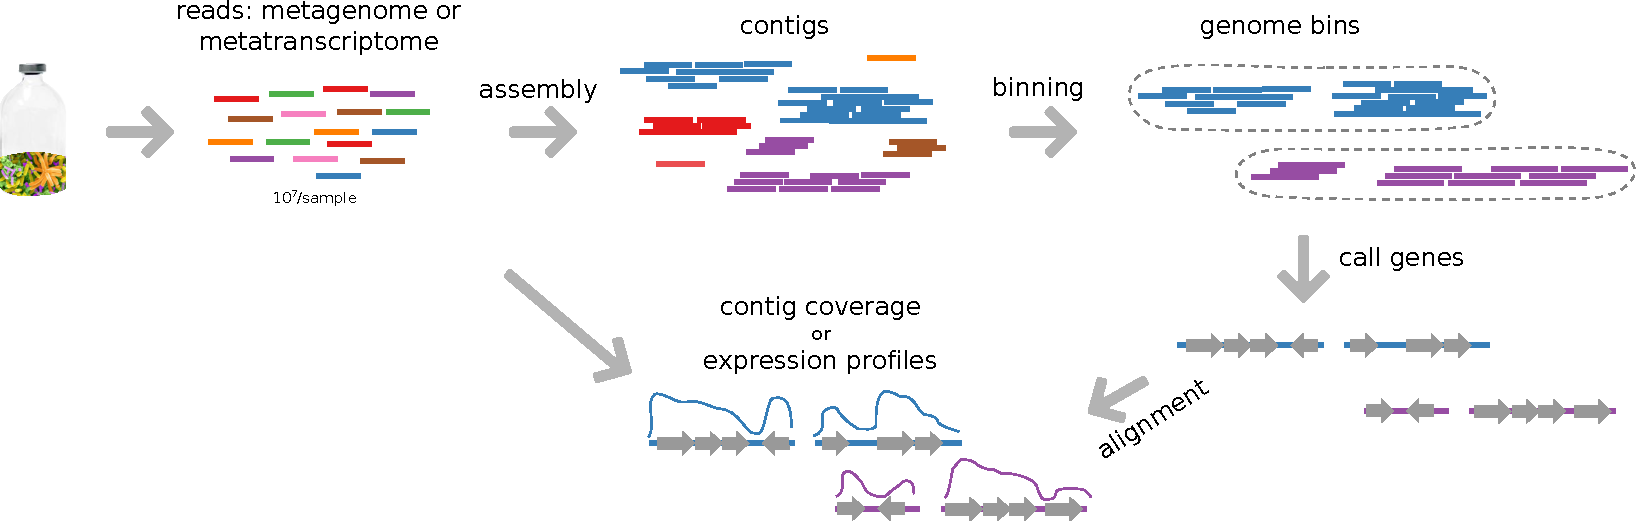
\includegraphics[width=1.0\textwidth]{./tex/chapter2/figures/170312_metagenomics_metatranscriptomics_overview.pdf}
    \begin{singlespace}
    \caption[Overview of elements in metagenomics/metatranscriptomics workflows]{
       Graphical introduction to basic vocabulary and inference steps of metagenomics and metatranscriptomics workflows.
	   Short colored lines = single reads, long colored lines = contigs,
	   gray arrows on top of colored lines = gene calls, wiggly lines above contigs depict the coverage of an alignment.}
    \label{fig:meta_workflow}
    \end{singlespace}
\end{figure}

A simplified representation of steps common to most shotgun metagenomics papers is depicted by Figure \ref{fig:meta_workflow}.
The first step of reference-free metagenomics is assembly, wherein contigs are aligned and fragments are merged to infer the sequence from which the reads originated.
Binning aims to identify contigs that in aggregate represent single organisms, or groups of highly related organisms \cite{kunin2008}.
Genes can be called on the contigs, either before or after binning, to reveal the genetic potential of the organisms.

The flow of information through metagenomics pipelines can be thought of as liquid flow through piping with leaks (Figure \ref{fig:pipe_leaks}).
In the process of aggregating information, each software step can lose information ("leak") along the way.
Flow (read accountability) can be measured at the input and exit of pipes (represented by flow gauges), allowing identification of how well output data reflects the original samples, and at which step(s) information was lost.

\begin{figure}[H]
\centering
    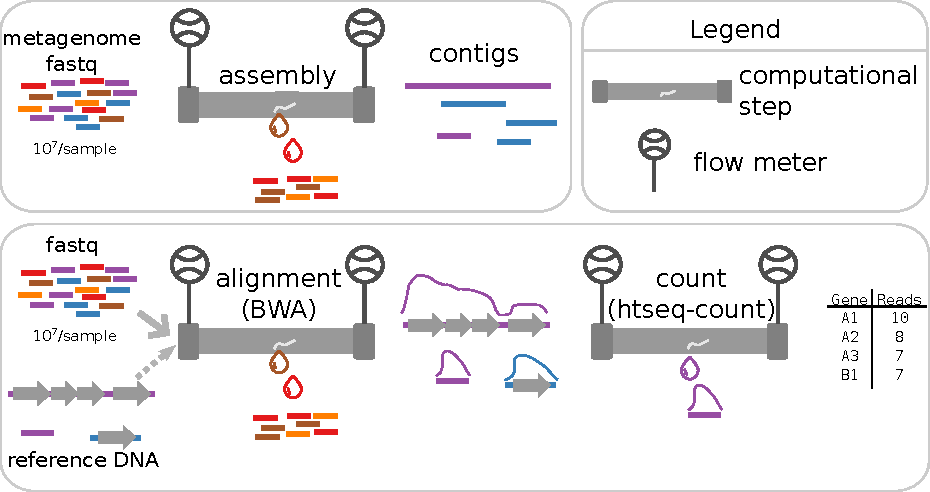
\includegraphics[width=0.8\textwidth]{./tex/chapter2/figures/170312_pipe_leaks.pdf}
    \begin{singlespace}
    \caption[Framework for assessing information loss in workflow steps]{
        Cartoon representing the ability to deduce information loss at different steps of the metagenome/metatranscriptome work flow.}
    \label{fig:pipe_leaks}
    \end{singlespace}
\end{figure}

%---- Pipe description
%A simplified cartoon of the framework used to assess efficacy of each tool in the work flow is illustrated by Figure \ref{fig:pipe_leaks}.
For papers where the goal is to describe one or several novel organism(s) with high confidence, the loss of information (reads) along the way may not be a significant concern.
Often papers in this category do not clearly report estimates of the abundance of these organisms in the natural community.
% Don't trash other papers \cite{evans2015} , or obscure absolute abundances by using relative abundances \cite{daly2016}.
Other papers try to describe a more wholistic description of the community (e.g. \cite{kantor2017}) by describing the diversity of organisms identified via binning.
In this case, it is crucial to quantify what fraction of the original sample is described by the output of the computational analysis.
These statistics are usually not stated clearly, allowing readers to over-estimate the importance of the described taxa in the ecosystem.
% At this stage, or research is in this camp, and the result section will highlight how this frame of mind guided selection of tools.
The pipe analysis framework illustrates the approach of this paper: use multiple monitoring methods to determine which pipeline steps are associated with information loss.
These statistics are assessed throughout to prevent misinterpretation of claims about community compositions and expression patterns.
%This thesis aims to describe the community wholistically, and thus strives to clearly report assembly, binning, and read mapping efficacy so as to not overstate claims or exaggerate community simplicity.
% Many literature studies report small and incomplete descriptions about efficacy of their assembly and binning, which obfuscates leaks in the analysis pipeline and corresponds to over-simplified descriptions of the environment under study.  % Don't cite: hard to be certain I read carefully enough to call out papers by name.  It's also not nice!

%----- There is no road map!
Each computational step can be executed by several or sometimes dozens of competing software packages \cite{sangwan2016,thomas2012}.
Each tool can report basic statistics about efficacy based on inputs and outputs, but it it up to the researcher with larger-scope understanding of the project goals to write scripts to critically assess efficacy of the tools in aggregate.
Results from one software package can give you better insight about how to evaluate the results of other packages, so an iterative process with various somewhat-equivalent tools can maximize accuracy.

Another challenge of projects of this scope is the size of the data.
While more data can lead to greater potential for extracting information from uncertain data, many tools are not designed to work on sequencing data as large as these.
While some tools fail quickly and with informative messages, other simply fail by running indefinitely without the tool either completing its task or aborting.
For some goals, the data can be broken into subsets, processed separately, and re-joined upon completion.
However, not every tool can operate on segments of the data, and extra care is required when stitching together results so the next tool downstream will be blind to the upstream manipulations.

%Tools choke.  Just don't complete.
%Sometimes the parameters can be altered, sometimes you can break up a dataset and feed it to a tool in pieces, but sometimes the size is a deal breaker.

It is the role of the computational biologist to learn enough about the competing tools to select a handful to try, develop metrics and priorities for the trade-offs of each tool, project complex data into summary graphs, and decide which tool is the best fit for the research goals.

\subsubsection{Assembly}
%---- Why assemble
Analysis of metagenomic and metatranscriptomic data usually beings with assembling metagenome reads into contigs (Fig \ref{fig:meta_workflow}), which are contiguous stretches of genomic sequence in which the order of bases is known to a high confidence level. %(JGI)
The metagenomes can be aligned to these contigs to infer the abundance of organisms.
The transcriptomes can be aligned to these same contigs to infer what genes are expressed.
In principle, metagenomes and metatranscriptomes can be aligned to isolate genomes rather than contigs, however, in practice meta-omics experiments are usually used precisely when the isolates available are known to be incomplete representatives of the microbial community under study.
Even if a similar organism has been isolated, the investigation may be probing the diversity of similar organisms, or the influence of less abundant microbes on the function of the community.

%---- Not all assemblies are created equal
The challenge of assembly scales with the complexity of the microbial community.
High species diversity and strain-level heterogeneity add challenge to assembly \cite{kunin2008, thomas2012}.
Communities with a small number of well-delineated species tend to assemble better, yielding shorter numbers of long contigs.
In contrast, the high diversity of complex communities can lead to fragmented assemblies that have fewer long contigs and more short contigs \cite{kunin2008}.
These shorter contigs are more challenging to analyze and can lead to an incomplete portrait of a community.
Short contigs are more difficult to call genes on, and are also more difficult to bin because measures like GC and differential abundance are noisier for short contigs than long ones \cite{sangwan2016}.
The most common measures of assembly efficacy are characteristics of the contigs themselves.  How many are there?  What is the length of the contig that divides the length-sorted contigs into a pair of equal lengths (termed "N50")?
This thesis advocates for additional measures that are rarely reported: the fraction of the total (un filtered/trimmed) original reads that map to the assembled contigs, and genome bins.   % todo: "seldom seen" instead of "not seen"?
% Dont' talk about restricting to contigs > 1.5kb.

\subsection{Elviz Assemblies}
%---- JGI assemblies
The sequencing for many metagenomics projects, including this one, are done by the Joint Genome Institute (JGI).
JGI provides some bioinformatics processing in addition to providing un-processed reads.
The software they run assembles contigs for each sample individually, predicts genes, and calls taxonomy for contigs \cite{cantor2015}.
They also report the number of reads and average coverage for each contig.
These measures are a great starting point for answering "who's there" in terms of taxa abundance, but does neglect information about reads that did not assemble well and thus must be used with caution.

%---- Not assembled together
The contigs JGI provides are assembled for each sample, individually.
For this project, that means there are 88 separate assemblies.
Thus the contigs are not shared across samples, and comparison across samples is hindered.
For example, it is difficult to infer whether a particular gene is differentially expressed across two samples if the contigs used as reference DNA are not the same across samples.
More powerful analyses can be done when the DNA from all metagenomic samples are assembled together.
This makes it possible to map DNA and RNA reads back to this shared DNA and thus to tabulate gene expression across samples.
Such an assembly also leads to more powerful binning (discussed below) by providing extra features to cluster with: the differential abundances of each contig across the samples \cite{albertsen2013}.
Since the number of reads originating from a particular organism should be proportional to its abundance, the DNA coverage for a set of contigs originating from an organism should be similar in a particular sample, and correlated across samples.
The per-sample nature of the JGI contigs restricted the types of analyses that data was used for, and motivated generation of co-assembled contigs to represent the entirety of the dataset as discussed below.

\subsubsection{Binning}
%---- Definition & Why
Desire for understanding at organism-level often leads investigators to approximate genomes as best they can from a set of metagenomic contigs.
The phrase "genome bin", often called simply "bin", is used to describe a collection of contigs used to approximate the genome of a single organism.
"Bin" implies the collection is expected to be somewhat incomplete and potentially contaminated by DNA of other strains or species.
Bins allow inference of which metabolic pathways are available, and can be used as a reference to map RNA to for quantification of how these genes are expressed.
Higher confidence claims would be possible upon isolation of the organism represented by the genome bin, but laboratory isolates are often not obtainable either due to obligate partnerships with other organisms, or a variety of intolerances to laboratory conditions \cite{stewart2012}.
Binning can be done before or after annotating genes on the contigs, as very few methods use gene calls in the binning process.

%---- Overview of binning tools' strategies
The most common features used to bin contigs include GC content, tetranucleotide frequency, other oligonucleotide frequencies, and differential abundance across samples \cite{sangwan2016}.
Most aim to be effective without needing reference genomes to align to.
% can't find citation for using an isolate as a binning reference.  Only for assembly.  Drop??

%---- Rarefaction, species heterogeneity
The ability to get clean genome bins varies greatly from project to project.
As with assembly, more rarefied samples with low levels of strain heterogeneity are more amenable to binning \cite{kunin2008, thomas2012}, as the contigs are more likely to be long and few in number.
Longer contigs have reduced noise for measurements of GC ratio, tetranucleotide frequency, and differential abundance \cite{sangwan2016}.
This in turn leads to less ambiguity when sorting contigs into respective bins.
Notably, most binning tools are demonstrated on simple communities such as the premature infant gut \cite{sharon2013}.
Thus, the promising assembly quality statistics noted in binning method papers are not guaranteed to translate for analysis of high-complexity samples such as those in this thesis.
% In fact, most binning methods were demonstrated using relatively simple communities (e.g., premature infant gut datasets of Sharon et al.

%---- Bin assessment
The quality of bins can be determined using metrics of completeness, contamination, and efficacy of representing the sample.
Completeness and contamination checks can be automated by use of CheckM \cite{parks2015}, which uses the presence of marker genes in each bin as the basis for its approximations.
The marker genes used by CheckM are different based on the approximate taxonomy CheckM infers for the bins.
While this is certainly more effective than one set of genes used for all microbes, the reference sets available may not be good fits for the particular microbes under study.
Furthermore, the choice of reference gene sets might be poor for messy bins that contain contigs from wildly different taxa.
Some papers determine completeness and contamination by manual inspection using domain-specific marker gene sets. % (cite)
For papers published before CheckM, this manual check was the best option.
Now CheckM is used in the majority of papers.
It even allows the possibility of adding custom marker gene sets for CheckM to use.

%---- Binning tools
The binning tools used herein combine sequence composition and coverage across multiple samples as inputs to machine learning algorithms that automatically cluster contigs into genomes.
Several were tried, given that differences in their algorithms and output characteristics are seldomly and vaguely reported \cite{sangwan2016}.
Metabat \cite{metabat2015} uses k-medoid clustering of a distance measure composed of tetranucleotide frequency and abundance.
% ** doesn't use marker genes **
MyCC \cite{mycc2016} uses affinity propagation to cluster contigs, and uses the presence of marker genes to correct clusters.
%"an automated binning tool that combines genomic signatures, marker genes and optional contig coverages within one or multiple samples"
%"FetchMG extracts 40 universal phylogenetic marker genes"
%"AP-generated clusters were finally corrected based on the sequences harboring marker genes"
CONCOCT \cite{concoct2014} uses a Gaussian mixture model fit with a variational Bayesian approximation, on features thinned out via principle components analysis (PCA).
% This says it uses marker genes, but the original paper doesn't mention it.
% Manual curation
Almost every high-quality bin published in high-profile papers has used tools such as these, but the resulting bins are subsequently refined by manual curation, with methods only vaguely described.

\subsubsection{Mapping RNA}
Metatranscriptomes can be mapped to contigs or bins.
A key variable to consider is what you want to happen with reads that map to multiple places.
If a read maps equally well to two different contigs in a bin, should it be randomly assigned to one locus, or thrown away?
If the study is aiming for differential expression type analysis, than the latter is better.
Discarding ambiguous reads is the default of most alignment and counting tools.
If the study aims to describe a wholistic picture of expression in a sample, it may be worth guessing the source of multiply mapped reads.
Special care must be taken after that step, as the estimates will certainly be wrong some of the time.


%==========================================================================================================================================
%==========================================================================================================================================
%==========================================================================================================================================
\section{Methods}

\subsubsection{Experimental}  % Note that work was done previously, so I'm not implying I did it.
The culturing and sample preparation was done by Maria Hernandez, a visiting scholar.
Sediment stored in an aqueous DMSO solution on previous sampling trip was thawed from -80$^o$C and distributed into 250 mL bottles containing 100mL of NMS medium \ref{fig:experimental_design}, leaving 150mL of headspace.
% High: 75% air, low = 75% air.  150 mL headspace, 100 mL liquid.
All bottles were air-tight, with head spaces containing 25\% methane.
The high \ce{O_2} samples had 75\% air in the head space.
The low \ce{O_2} samples had 15\% air in the head space, with the remainder being nitrogen.
Atmospheres were created every weekday and once per weekend.
Bottles were shaken at 250 RPM and held at 18$^o$C.
The gaseous compositions for the days between transfers were not measured.

Bottles were serially transferred for 14 weeks.
Metagenomes and metatranscriptomes were obtained for all samples corresponding to weeks 4-14.
Earlier weeks were omitted due to potential effects of residual DMSO, and interest in prioritizing sequencing of later, more-rarefied samples.
The \ce{O_2} conditions (low/high) were switched for the last 4 bottles in each series (see Figure \ref{fig:experimental_design}).

\subsubsection{Sequencing}
This large dataset was made possible by a Joint Genome Institute sequencing grant. % (cite the \#? XX).
JGI sequenced all samples on an Illumina platform to produce the 88 metagenomes and 88 metatranscriptomes.
Ribosomal RNA was removed before sequencing the metatranscriptomes.
%~ XX (?? Paired ended?) reads per sample, for both metagenomes and metatranscriptomes (??).

\subsubsection{Elviz Analysis}
Along with raw sequencing outputs (\texttt{fastq.gz} files) for each sample, Elviz data \cite{cantor2015} was provided by JGI.
These data included one assembly per metagenome, corresponding contig statistics, and transcriptome alignment statistics.
In addition, they provide taxonomy for each contig, to some degree of certainty: some are only labeled to the kingdom level, whereas others are specified all the way to genus.
The taxonomy, contig lengths, and number of reads mapped to each contig were used to infer the distribution of taxa in each sample.
The metric used was the fraction of reads assigned to contigs with the specified taxonomy (code at \url{https://github.com/JanetMatsen/elvizAnalysis/blob/master/abundance_utils.py}).
Length of contigs was not normalized out, or the abundance of short contigs would dominate the results.
The code checks that the taxas` abundances summed to 1 for each sample.

Tools were written to aggregate (a) based on taxonomy level, or (b) everything below a taxonomy level.
Contigs with taxonomy not described to the specified level were grouped into "unknown \& other".
This framework was also used to summarize abundances at mixed taxonomy level (e.g. phylum Bacteroidetes, order Burkholderiales, family \textit{Methylococcales}, and family \textit{Methylophilales}), and plotted (code: \url{https://github.com/JanetMatsen/elvizAnalysis/blob/master/abundance_plot_utils.py}).

Statistics for the 88 samples were merged with information about the \ce{O_2}, replicate, and week values corresponding to each sample using Python and Pandas.
Plotting was done with Matplotlib, Pandas, and Seaborn.

\subsubsection{Computational resources}
This computationally-intensive research was supported by an AWS research grant, which included \$27k of compute resources and expert consulting on how to best utilize the vast services offered.
AWS allows per-hour rental of machines with different specifications, that the user can choose based on algorithm needs.
Furthermore, the ability to share machine images with other researchers greatly facilitates the potential reproducibility of research.
Upon project completion, an Amazon Machine Image (AMI) encapsulating the entire data analysis pipeline will be provided so others can re-run our analyses.

The machine ("instance") type used in all methods to follow was an AWS EC2 c4.8xlarge instance, which has 36 cores and 60GB memory.
This was sufficient for all work, other than the memory-intensive assembly step, as noted below.
Instances could be turned on and off as needed, reducing compute costs.
This is in contrast to sharing a similar machine with an entire research lab, which would have slowed down analysis and caused conflicts when certain computations used all of the compute resources, sometimes causing computer failure.

Each instance obtained data and wrote results to a shared file system.
The 9 TB of data, scripts, and results were stored using the AWS Elastic File System (EFS).
EFS is currently the most versatile and highest performance (most expensive) file storage available within AWS, which allows users to have multiple instances reading/writing to the same directory.
This shared nature of the files allows the user to spin up a second computer instance as needed, and do read/write operations on the exact same set of files.

%---- Computation parallelization
Parallelization of compute tasks was done by splitting jobs across a single large computer, or across separate EC2 instances.
When tasks were parallelized across one powerful computer, Gnu parallel or Python \texttt{pool.map} was used.
When parallelizing across more, often weaker, computers, an AMI was made that mounts the EFS-stored data.
These instances were usually started by hand through the console, though proof of principle studies using the Amazon Command Line Interface (CLI),
    and an Autoscaling/SQS service pair were explored to set the foundation of future work (see repository \url{https://github.com/JanetMatsen/AWS_parallel_Cowsay}) for the templates developed.

\subsubsection{Map to isolate genomes}
As a preliminary study, the metatranscriptomes were mapped to 55 genomes (Table \ref{table:55genomes}) isolated from Lake Washington by the Lidstrom Lab.
The sequences were downloaded from NCBI, and concatenated together before mapping.
Mapping to the multi-fasta rather than the individual genomes prevents double-counting of reads that map well to multiple loci.
BWA-MEM \cite{li2009} with default settings was used to map each transcriptome to the multi-fasta, and htseq-count \cite{anders2014} was used to tabulate expression estimates.
Samtools \cite{li2009samtools} was used to evaluate mappings produced by BWA-MEM.
Note: the default of BWA-MEM is to flag reads that map equally well to two or more loci as having quality score 0; htseq-count by default omits these counts from the table of reads per gene (discussed later).

\begin{singlespace}
\begin{longtable}{p{.50\textwidth}}
\caption[The 55 isolate genomes used]
	{The 55 isolate genomes used.}
\label{table:55genomes}
\endfirsthead
\endhead
\midrule
               \textit{Ancylobacter} sp. FA202 \\
                 \textit{Arthrobacter} sp. 31Y \\
                 \textit{Arthrobacter} sp. 35W \\
               \textit{Arthrobacter} sp. MA-N2 \\
                    \textit{Bacillus} sp. 37MA \\
                      \textit{Bacillus} sp. 72 \\
                        \textit{Bosea} sp. 117 \\
                \textit{Flavobacterium} sp. 83 \\
                \textit{Flavobacterium} sp. Fl \\
                      \textit{Hoeflea} sp. 108 \\
               \textit{Hyphomicrobium} sp. 802 \\
                \textit{Hyphomicrobium} sp. 99 \\
           \textit{Janthinobacterium} sp. RA13 \\
    \textit{Methylobacter tundripaludum} 21/22 \\
    \textit{Methylobacter tundripaludum} 31/32 \\
              \textit{Methylobacterium} sp. 10 \\
              \textit{Methylobacterium} sp. 77 \\
             \textit{Methylobacterium} sp. 88A \\
                \textit{Methylocystis} sp. LW5 \\
                 \textit{Methylomonas} sp. 11b \\
                \textit{Methylomonas} sp. LW13 \\
                 \textit{Methylomonas} sp. MK1 \\
        \textit{Methylophilaceae bacterium} 11 \\
                 \textit{Methylophilus} sp. \#1 \\
                 \textit{Methylophilus} sp. 42 \\
                  \textit{Methylophilus} sp. 5 \\
                 \textit{Methylophilus} sp. Q8 \\
                  \textit{Methylopila} sp. 73B \\
                 \textit{Methylopila} sp. M107 \\
            \textit{Methylosarcina lacus} LW14 \\
                 \textit{Methylosinus} sp. LW3 \\
                 \textit{Methylosinus} sp. LW4 \\
                 \textit{Methylosinus} sp. PW1 \\
            \textit{Methylotenera mobilis} \#13 \\
           \textit{Methylotenera mobilis} JLW8 \\
               \textit{Methylotenera} sp. 1P/1 \\
                \textit{Methylotenera} sp. 73s \\
                \textit{Methylotenera} sp. G11 \\
               \textit{Methylotenera} sp. L2L1 \\
                \textit{Methylotenera} sp. N17 \\
          \textit{Methylotenera versatilis} \#7 \\
        \textit{Methylotenera versatilis} 301, \\
          \textit{Methylotenera versatilis} 79 \\
           \textit{Methyloversatilis} sp. FAM1 \\
       \textit{Methyloversatilis} sp. RZ18-153 \\
   \textit{Methyloversatilis universalis} FAM5 \\
 \textit{Methyloversatilis universalis} Fam500 \\
   \textit{Methylovorus glucosetrophus} SIP3-4 \\
                \textit{Mycobacterium} sp. 141 \\
                \textit{Mycobacterium} sp. 155 \\
                    \textit{Paracoccus} sp. N5 \\
               \textit{Pseudomonas} sp. 11/12A \\
                 \textit{Xanthobacter} sp. 126 \\
                  \textit{Xanthobacter} sp. 91 \\
     \textit{Xanthobacteraceae bacterium} 501b \\
\midrule
\end{longtable}
\end{singlespace}


\subsubsection{Assembly} % (Dave)
Assembly to produce contigs was done on pooled quality-trimmed metagenome reads via Megahit \cite{li2015}.
This memory-intensive computation was done on an AWS instance with 1 TB of memory.
Assembly of multiple samples simultaneously provides a shared set of contigs to use when mapping DNA reads or RNA-seq reads from any of the 88 samples.  % Not methodsy?  Take out?  TODO
This in turn allows for comparison of gene expression across samples.
The fraction of reads represented by the assembly, in aggregate, were measured to verify assembly efficacy.
%Tune knobs until ...
%Followed protocol ...

\subsubsection{Gene calls}
Genes were called on contigs with length greater than or equal to 1.5kb using Prokka \cite{seemann2014} (scripts: \href{https://github.com/BeckResearchLab/meta4/blob/master/m4b_binning/assembly/prokka/prokka.py}{Python script} that calls Prokka, \href{https://github.com/BeckResearchLab/meta4/blob/master/m4b_binning/assembly/contigs_by_length/select_contigs_by_size.py}{script} that extracts contigs by size).
This cutoff was selected because shorter contigs are not recommended for inclusion by most binning tools documentation.
Additionally, shorter contigs are less likely to have genes identified on them, as genes are more likely to be incomplete due to a higher density of contig edges.
Prokka did not tolerate an input size of the scale, so the input fasta was broken into 5 files of approximately equal size (\href{https://github.com/BeckResearchLab/meta4/tree/master/m4b_binning/assembly/prokka/contigs}{scripts}).
These were processed in parallel, using the \texttt{pool.map} function of Python.
A \href{https://github.com/BeckResearchLab/meta4/blob/master/m4b_binning/assembly/prokka/contigs/glue_together_gffs.py}{script} was written to merge the resulting annotated "general feature format" files (\texttt{.gff} files) into one representing all contigs $\geq$ 1.5kb.

\subsubsection{Checking the ability of contigs to represent each metagenome}
The loss of information resulting from omitting short contigs was assessed by counting the number of reads that map to contigs $\geq$ 1.5kb, and comparing that to the total number in the raw metagenome \texttt{fastq.gz} files (\href{https://github.com/BeckResearchLab/meta4/blob/master/m4b_binning/assembly/data/sample_info/count_reads_in_each_sample.sh}{\texttt{.fastq} read counting script}, \href{https://github.com/BeckResearchLab/meta4/tree/master/m4b_binning/assembly/assess_sample_mappings_to_contigs}{analysis}).
This represents an upper bound in information content for the assembly step.
Again, this used BWA-MEM \cite{li2009}, and a \href{https://github.com/BeckResearchLab/meta4/blob/master/m4b_binning/assembly/data/sample_info/count_reads_in_each_sample.sh}{script} written to count reads in \texttt{.fastq} files.
Pandas (Python) was used to merge results together.

\subsection{RNA-seq: mapping to contigs $\geq$ 1.5 kb}
Like all other read mapping steps, transcriptomes were mapped with BWA-MEM (default settings), and per-gene results were summarized with htseq-count.
Contigs $\geq$ 1.5kb were used as reference DNA.
Metatranscriptomes were mapped to these contigs all at once, rather than to each bin individually in order to reduce over-counting.
This does result in reads mapping identically well to two places being thrown out, as mentioned earlier.
Results from each sample were merged using a 60GB RAM AWS instance, rather than SQL.
The fraction of transcriptome reads was compared to the total number in the input \texttt{.fastq} files as a metric of information loss.
See \href{https://github.com/BeckResearchLab/meta4/tree/master/rnaseq/alignments}{scripts and notebook}.

\subsubsection{Binning}

Binning of contigs into genome-like bins was explored using three different packages.
MetaBAT was used with default settings on contigs $\geq$ 1.5kb (\href{https://github.com/BeckResearchLab/meta4/blob/master/m4b_binning/assembly/2.metabat}{script}).
As promised by the documentation, it scaled well to this large dataset. % and completed within about a day.

MyCC was used, but did not scale this large data set.
The large memory requirement of the underlying affinity propagation algorithm led to failures when default settings were used.
At one time, MyCC wrote so many small files that the machine crashed due to running out of inodes.
The authors suggested some alterations to the settings to reduce the computational requirements:  \texttt{56mer, lt 0.4, st 50}.
Use of their settings worked on the set of contigs longer than 2.5kb, but not the larger set of contigs longer than 1.5kb.

Concoct was tried initially, but bins were never obtained.
This tool reports multiple potential clusters per conitg.
The approach for resolving that conflicting information was not sorted out in the time frame of this project.

\subsubsection{Average Nucleotide Identity}
Average nucleotide identity (ANI) was used to compare bins.
The underlying tool, provided by JGI  \cite{varghese2015} (\href{https://ani.jgi-psf.org/html/anicalculator.php}{download link}), calculates two-way global ANI measures and reports the fraction of each genome that aligned.
The authors suggest removal of ribosomal RNA genes, which can have high ANI even for divergent organisms.
They do not, however, provide options or suggest a tool for this step.
Given that the ANI calculations intended only to give a rough idea of similarity between bins or bins and isolates, this step was not performed.
The tool was used to assessed ANI between all pairs of isolate genomes and MetaBAT bins (\href{https://github.com/BeckResearchLab/meta4/blob/master/m4b_binning/assembly/ANI/ANIs_of_all_combos.py}{script}).

\subsubsection{Additional bin characterization}

Completeness and contamination were checked with CheckM \cite{parks2015} (\href{https://github.com/BeckResearchLab/meta4/tree/master/m4b_binning/assembly/bin_info}{scripts}).
CheckM uses marker genes from what it determines to be an evolutionarily similar microbe.
The tool was benchmarked on isolates, to ensure it performed well on the key methylotrophic taxa under study.
Custom marker genes specific to methylotrophs were not added, however, this is suggested as a possible future direction to assess bins.

Taxonomy was approximated using PhyloPhlan \cite{segata2013}, and by ANI similarity with isolate genomes (\href{https://github.com/BeckResearchLab/meta4/tree/master/m4b_binning/assembly/bin_info}{scripts}).

\subsubsection{Code}
The code described was developed with Git version control, and the full history is available on GitHub:
\begin{itemize}
    \item \textbf{ElvizAnalysis}: \url{https://github.com/JanetMatsen/elvizAnalysis}
    \item \textbf{meta4} (assembly, binning, etc.): \url{https://github.com/BeckResearchLab/meta4}
\end{itemize}

%==========================================================================================================================================
%==========================================================================================================================================
%==========================================================================================================================================
\section{Results and Discussion}


%-------- Elviz Analysis
\subsection{Raw Reads}

The cumulative number of raw and un-filtered reads is shown below.
This collection of reads was used for all inferences described in this chapter.
Also see Figure \ref{fig:fastq_reads} for plots showing specific values for each sample.

\begin{table}[H]
% /work/misc/170326_compare_raw_fastq_reads.ipynb
\centering
\begin{singlespace}
\caption[Number of un-filtered reads: sample average and total]
	{Number of un-filtered reads: sample average and total across 88 samples.
	}
\begin{tabular}{l | cc}
 %\toprule
        & mean \# reads per sample & total \# reads \\
\midrule
	metagenomes & \texttt{3.33e+07} $\pm$ \texttt{7.34e+06} & \texttt{2.93e+09} \\ % also from: /work/jmatsen/170308_assess_Elviz_read_attraction_frac
	metatranscriptomes & \texttt{4.24e+07} $\pm$ \texttt{6.22e+06} &  \texttt{3.73e+09} \\
%\bottomrule
\end{tabular}
\label{table:sample_read_sizes}
\end{singlespace}
\end{table}



%-------- Elviz Analysis
\subsection{Elviz Analysis}

The best measure of which taxa dominate the samples comes from the Elviz \cite{cantor2015} data.
As described in the Methods section, the abundance measure was the sum of read counts across contigs labeled with the taxonomy of interest.
Traditional metrics like RPKM \cite{mortazavi2008} and TPM \cite{wagner2012} are excellent for comparing coverage or expression across features or samples, but could not be used due to the need to sum values across contigs.
To illustrate why length of contig could not factor into the abundance measure, consider this:
a contig with length 10kb should contribute nearly identically to an equally expressed second 10kb stretch of DNA that for technical reasons was assembled into two 5kb stretches rather than one 10kb contig.
Any scheme that controlled for contig length or was weighted by the statistic of each contig would skew the aggregated number down for metagenomic datasets such as this with many short, low-coverage contigs.
The fact that these assemblies are dominated by short contigs means that RPKM and TPM would bias the aggregate statistics toward the statistics of the shorter and less reliable contigs.
Similarly, median coverage was not used or the unreliable coverage numbers associated with short contigs would dominate the measure.

Figure \ref{fig:4dominant_groups} shows abundances of the four major taxonomic groups, Methylococcales, Methylophilales, Bacteroidetes, and Burkholderiales, according to the Elviz taxonomy calls for each contig. % Methylococcales, Methylophilales are Orders (not italics)
(Recall introductory Figure \ref{fig:taxonomy} for a hierarchical visualization of these taxonomies.)
Their dominance is consistent with pervious studies \cite{beck2013LW, beck2014LW, oshkin2015LW, hernandez2015LW, kalyuzhnaya2008Burkholderiales}.
Figure \ref{fig:dominant_genera} show the breakdown of the methanotrophic and non-methanotrophic methylotroph taxa in Figure \ref{fig:4dominant_groups}.
Notably, the path to rarefaction is not particularly consistent across samples.
Like previous studies, the dominant methanotrophic order/genus was Methylococcales/\textit{Methylococcaceae} and the dominant non-methanotrophic methylotrophic order/genus was Methylophilales/\textit{Methylophilaceae}.
Low \ce{O_2} was associated with a higher abundance of methanotrophs, and a lower proportion of methylotrophs than the high-\ce{O_2} samples.
\textit{Methylosarcina} is often found in high-\ce{O_2} samples, but rarely in low-\ce{O_2} samples.
Two high \ce{O_2} samples are dominated by \textit{Methylobacter}, but the others are not.
The last four samples in each series are more similar to the previous samples in the series than samples at the opposite \ce{O_2} tension.


\begin{figure}[H]
\centering
    % /Users/janet/elvizAnalysis/ipython_notebooks/plots/
    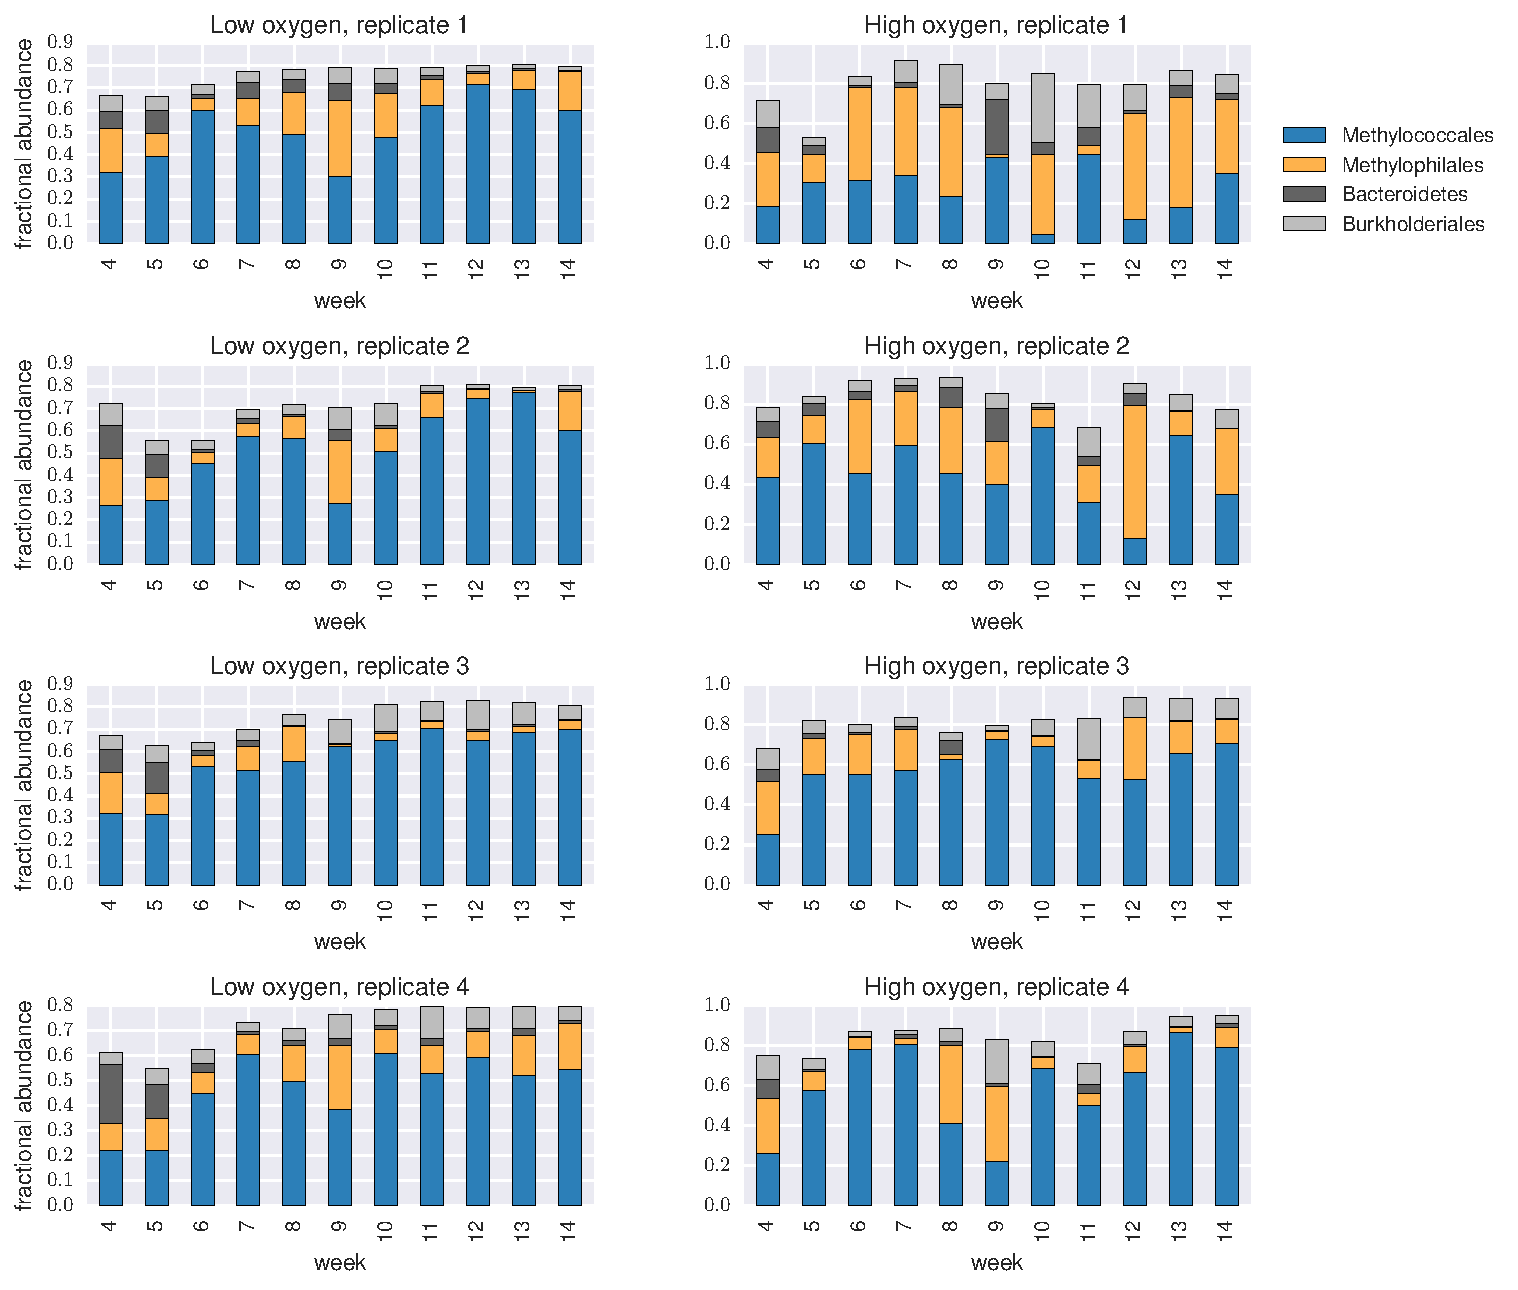
\includegraphics[width=1.0\textwidth]{./tex/chapter2/figures/170413_4_main_groups.pdf}  % ElvizAnalysis
    \begin{singlespace}
    \caption[Four major taxonomic groups in Lake Washington sediment incubations]{
        Fractional abundances of DNA from the four major taxonomic groups in Lake Washington sediment incubations:
	    phylum Bacteroidetes, orders Methylococcales (methylotrophs), Methylophilales (non-methanotrophic methylotrophs), Burkholderiales.
        The vertical gray line indicates the week the \ce{O_2} conditions were reversed.
        These bars only reflect reads that mapped to contigs, according to the Elviz pipeline.
        For information about the fraction of reads not assigned to contigs, see Figure \ref{fig:frac_elviz_mapped_to_contigs}.
        }
    \label{fig:4dominant_groups}
    \end{singlespace}
\end{figure}

\begin{figure}[H]
\centering
    % /Users/janet/elvizAnalysis/ipython_notebooks/plots/170313_methanotroph_methylotroph_taxa--portrait.pdf
    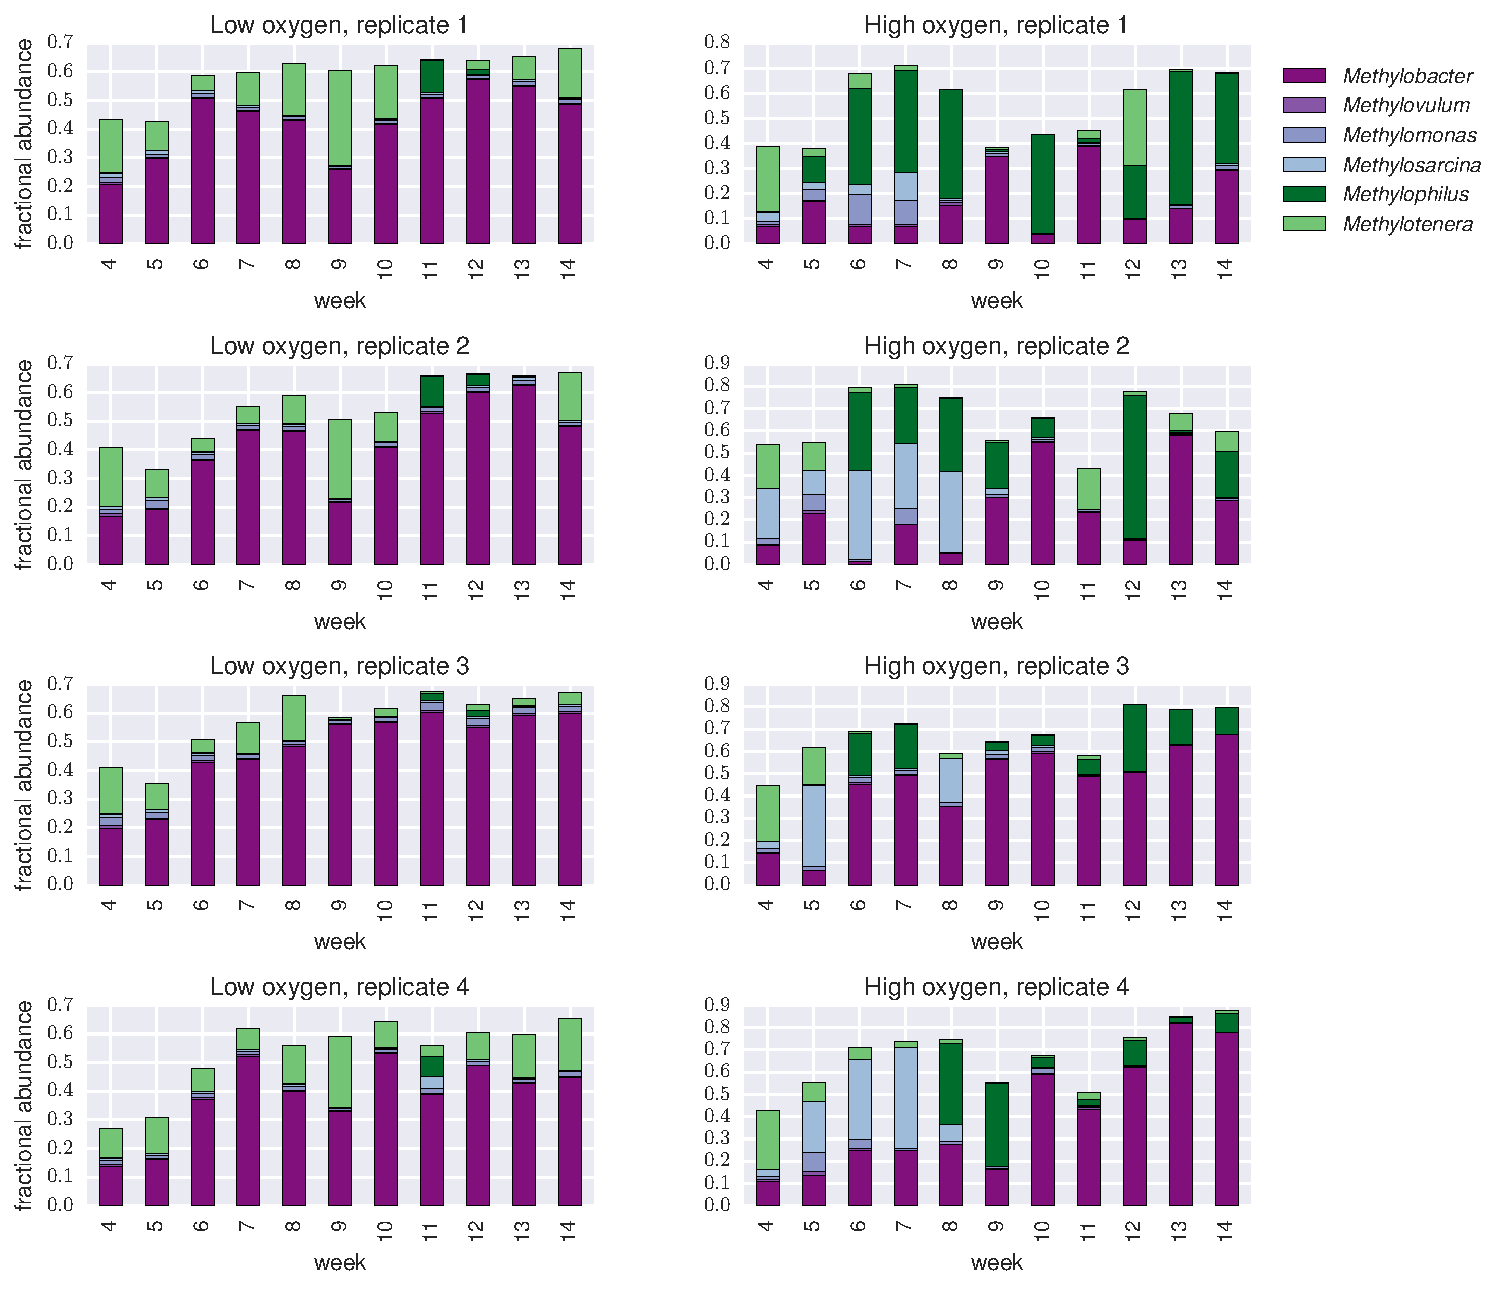
\includegraphics[width=1.0\textwidth]{./tex/chapter2/figures/170313_methanotroph_methylotroph_taxa--portrait.pdf}  % ElvizAnalysis
    \begin{singlespace}
    \caption[Dominant methanotrophic and methylotrophic genera]{
        Fractional abundance of DNA from the dominant methylotrophic genera.
        Purple bars are methanotrophs of order Methylococcales, family \textit{Methylococcaceae}
            (represents major taxa in blue bars of Figure \ref{fig:4dominant_groups}).
        Green bars are non-methanotrophic methylotrophs of order Methylophilales, family \textit{Methylophilaceae}
            (represents major taxa in yellow bars of Figure \ref{fig:4dominant_groups}).
        See Figure \ref{fig:taxonomy} for hierarchical taxonomy reference.
        Vertical gray line indicates the week the \ce{O_2} conditions were reversed.
        Like Figure \ref{fig:4dominant_groups}, these bars only reflect reads that mapped to contigs, according to the Elviz pipeline.
        For information about the fraction of reads not assigned to contigs, see Figure \ref{fig:frac_elviz_mapped_to_contigs}.
        }  % Italics are used for bacterial and viral taxa at the level of family and below.  https://wwwnc.cdc.gov/eid/page/scientific-nomenclature
    \label{fig:dominant_genera}
    \end{singlespace}
\end{figure}

\subsubsection{Binning Potential: Elviz Contigs}

%Genomic-scale resolution drove investigation of the potential for sorting these contigs into genome bins.
The goal of this study is a comprehensive description of the samples, ideally in terms of genome bins.
The potential for these Elviz contigs to paint a comprehensive picture of the microbial community was measured by summing all reads assigned to contigs long enough to bin, namely contigs $\geq$ 1.5kb.
Figure \ref{fig:dont_bin_Elviz} shows that while the entire set of contigs represents the samples well, the subset of contigs that are candidates for binning explain less than 20\% of the reads obtained for many low \ce{O_2} samples.
Another complication of binning these Elviz contigs, is that binning the contigs for each sample individually would lead to many redundant bins that need to be thinned.
This process is prone to human bias, and can lead researchers to over-fit their bins to their quality measures and thus over-state the quality of their bins.
Nonetheless, if a particular sample is enriched in an organism of interest, use of the contigs from that sample should be conisdered for future binning efforts.


\begin{figure}[H]
\centering
    % /Users/janet/Dropbox/meta4_bins_data_and_files/1703014_is_Elviz-_junk_revised/results
    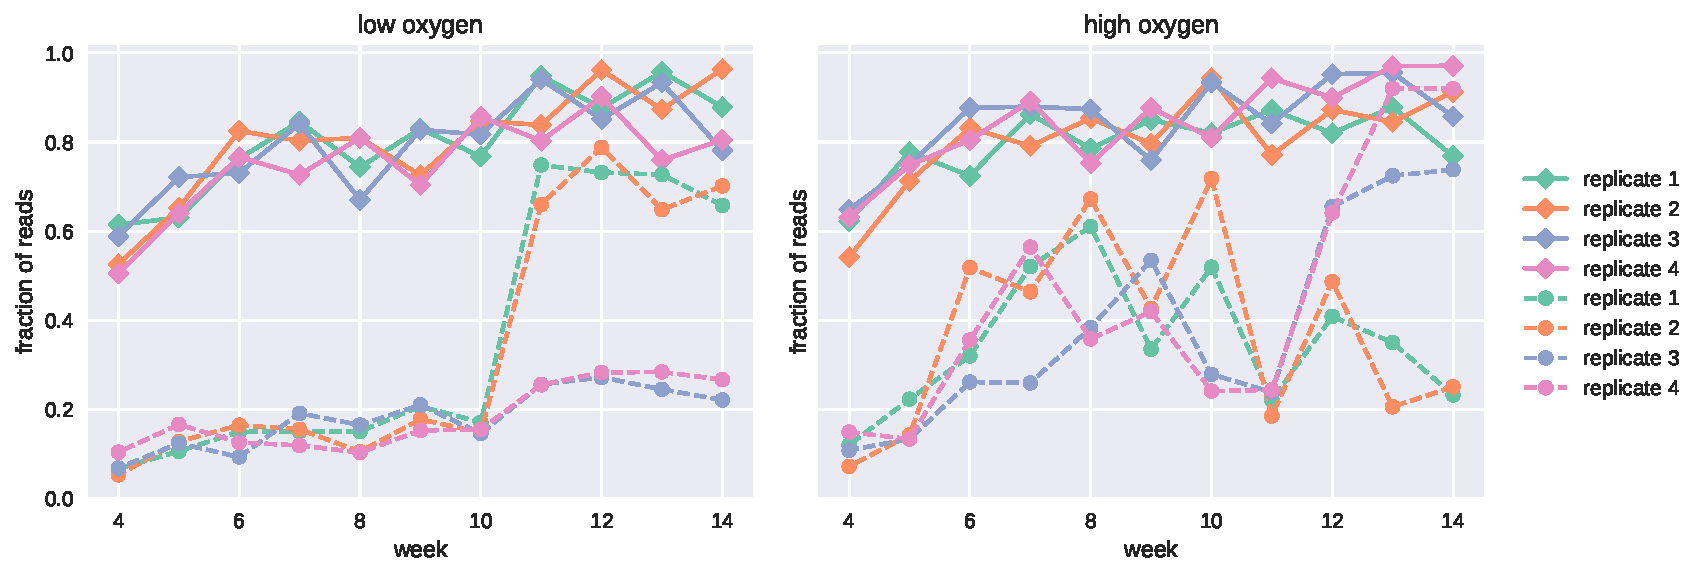
\includegraphics[width=1.0\textwidth]{./tex/chapter2/figures/170314_Elviz_is_not_for_binning--landscape.pdf}  % ElvizAnalysis
    \begin{singlespace}
    \caption[Upper-bound limit on success of binning Elviz contigs]{
        The upper-bound limit on success in binning Elviz contigs, as measured by the fraction of metagenome reads mapped to contigs.
        Lines are colored by replicate.
        Solid lines represent the fraction of reads in the raw \texttt{.fastq} file that map to contigs of any length.
        Dashed lines represent the fraction of reads in the raw \texttt{.fastq} file that map to contigs with length $\geq$ 1.5kb.
        Less than 20\% of the raw fastq reads would be explained by aggressive binning of most low \ce{O_2} samples.}
    \label{fig:dont_bin_Elviz}
    \end{singlespace}
\end{figure}

% ----- Map to Isolate Genomes ------
\subsection{Map to Isolate Genomes}

The next simplest approach for identifying which microbes are active in the samples, and what they express is to map the reads to the 55 isolate genomes (listed in Table \ref{table:55genomes}).
The potential efficacy of these results can be measured by quantifying the fraction of metagenomic and metatranscriptomic reads that align to these genomes (recall the pipe diagram, Figure \ref{fig:pipe_leaks}).
Figure \ref{fig:isolate_RNAseq} shows the fraction of the metatranscriptomes that can be explained using these reference genomes.
The low accountability (mostly $<$15\%) guarantees an incomplete portrait of the activity in these samples, so the data was not pursued further.
Despite heroic Lidstrom Lab efforts to isolate strains, the set obtained thus far does not cover the complexity seen in real samples.
This indicates missing taxa and/or dissimilarity between the isolated strains and the ones that dominate in nature.
While this method of describing gene expression was not pursued father, it provides a baseline fraction of RNA mapped for any subsequent metagenomic methods to beat.


\begin{figure}[H]
\centering
    % /Users/janet/Dropbox/thesis/tex/chapter2/figures/170208_fraction_of_transcriptome_reads_mapped_to_isolates.pdf
    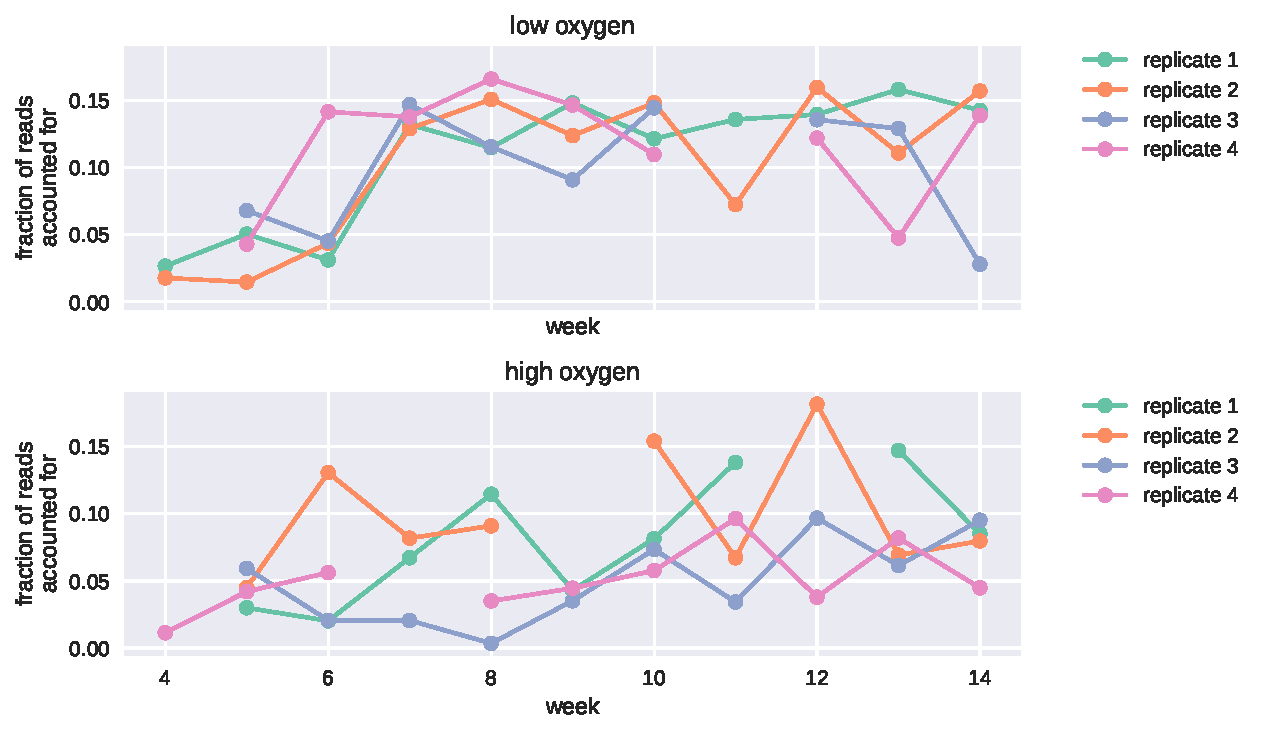
\includegraphics[width=1.0\textwidth]{./tex/chapter2/figures/170208_fraction_of_transcriptome_reads_mapped_to_isolates.pdf}
    \begin{singlespace}
    \caption[Measure of RNA-seq read accountability by isolate genomes]{
        Measure of RNA-seq read accountability by isolate genomes.
        Each dot represents the total fraction of raw reads assigned to genes when mapped to a concatenation of 55 isolate genomes.
        }
    \label{fig:isolate_RNAseq}
    \end{singlespace}
\end{figure}

As noted in the Methods, all computational steps using BWA-MEM and Samtools use default handling of reads that map equally well to multiple places.
This leads to omission of multiply-mapped reads.
Such handling is the best-practice approach for differential abundance analysis, which is the most common workflow for the tools used.
It does, however, lead to under-estimation of gene expression levels and lower accountability of the original fastq reads. % TODO: cite
Higher mapping fractions could be achieved by randomly assigning reads to one target from the set of best potential targets, but this lowers uncertainty about which genes/organisms are most influential in the samples.


% ----- ASSEMBLY ------
\subsection{Assembly}

Given that the Elviz contigs and isolate genomes proved ineffective as reference DNA for comparative analysis of samples, a single set of contigs that could be used to assess all samples was sought.
One workflow for explaining a set of metagenomic/metatranscriptomic samples includes co-assembly of metagenome reads, calling genes on the resulting contigs, mapping the transcriptomes to these contigs, and tabulating the expression levels.
Accordingly, the metagenomes from almost every sample were pooled and assembled into one set of contigs shared by all samples.

Assemblies which produce long contigs are desired, as longer contigs are easier to call genes on and cluster by similarity during binning.
Communities with extremely low complexity (just a few microbes co-existing) can yield long contigs with greater potential for being sorted into high-confidence genome bins. % which are often described by authors as genomes, rather than bins.
As complexity increases, reduced sequencing depth and homologous regions between organisms inhibit the formation of long contigs.
The distribution of contigs obtained (Figure \ref{fig:contig_lengths}) do not suggest a simple community.


\begin{figure}[H]
\centering
    % /Users/janet/Dropbox/meta4_bins_data_and_files/170124_current_metabat_analysis_figures/170123_frac_reads_binned_at_different_contig_lengths_and_total.pdf
    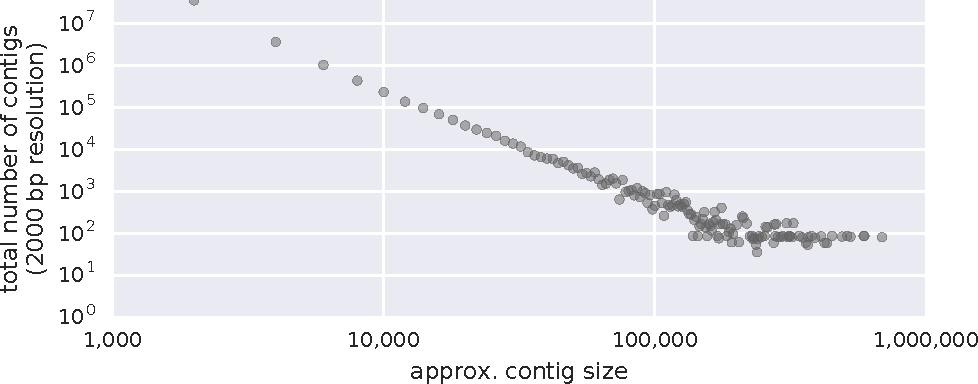
\includegraphics[width=1.0\textwidth]{./tex/chapter2/figures/170123_frac_reads_binned_at_different_contig_lengths_and_total--INKSCAPED.pdf}
    \begin{singlespace}
    \caption[Distribution of contig sizes]{
        Distribution of sizes for contigs assembled by MEGAHIT (2,617,225 contigs in total).}
    \label{fig:contig_lengths}
    \end{singlespace}
\end{figure}



% ----- ANNOTATION ------
\subsection{Annotation}

%[ec2-user@ip-10-0-0-158 map_to_contigs_longer_than_1500bp]$ realpath gene_read_totals.tsv
%/work/rnaseq/alignments/map_to_contigs_longer_than_1500bp/gene_read_totals.tsv
%[ec2-user@ip-10-0-0-158 map_to_contigs_longer_than_1500bp]$ cat gene_read_totals.tsv | wc -l
%107900

%[ec2-user@ip-10-0-0-158 map_to_contigs_longer_than_1500bp]$ realpath map_to_contigs_longer_than_1500bp_genes.tsv
%/work/rnaseq/alignments/map_to_contigs_longer_than_1500bp/map_to_contigs_longer_than_1500bp_genes.tsv
%[ec2-user@ip-10-0-0-158 map_to_contigs_longer_than_1500bp]$ cat map_to_contigs_longer_than_1500bp_genes.tsv | wc -l
%921436  % Includes 5 __ columns, use so 921,431.

Genes were called on contigs with length $\geq$ 1.5kb, in preparation for metatranscriptome studies (Table \ref{table:annotation}).
%Prokka identified 921,431 distinct genes, encoding 107,900 differently named proteins (Table XX).
See supplementary files for the gene \texttt{.fasta} and corresponding \texttt{.gff}. %, and RNA read counts \texttt{.tsv} in each sample.

\begin{table}[H]
\centering
\begin{singlespace}
\caption[Annotation of MEGAHIT contigs]
	{Annotation of MEGAHIT contigs.}
\begin{tabular}{l | c}
 %\toprule
        & statistic  \\
\midrule
	total \# of genes & \texttt{921,431} \\ % /work/jmatsen/170308_assess_Elviz_read_attraction_frac
	number of distinctly name genes & \texttt{107,900} \\
%\bottomrule
\end{tabular}
\label{table:annotation}
\end{singlespace}
\end{table}


% ?? Xox?

%Prokka was able to identify key methanotrophy/methylotrophy genes such as XXX.
%Some proteins were mis-annotated, as is typically observed when using automated annotation tools on methylotrophs.
%For example, many of the glucose dehydrogenases identified are in fact methane monooxygenases, and Xox-MDHs are listed as XXX.


% ?? TODO: make a plot that shows the gene density is lower on short contigs?


% ----- TRANSCRIPTOME ANALYSIS ------
\subsection{Transcriptome Analysis}

% Intro
Mappings of the 88 transcriptomes to the annotated contigs revealed which of the $\approx$0.9 million genes were strongly expressed.
Table \ref{table:top_genes} shows the names of the proteins associated with the highest total of reads mapped, and how many copies of each gene contribute to each sum.
See supplementary files (\texttt{.fasta}, \texttt{.gff}, and \texttt{.tsv}) for per-gene sequences, sequence information, and RNA-seq read counts by sample.

Figure \ref{fig:rna_mapping_bars} shows how well the called genes account for the transcripts seen in the raw sequence data.
The green bars represent a high degree of certainty.
Gray bars correspond to "no feature", which is presumably correlated to short contigs for which gene calls are less likely.
Pink bars are labeled as having low alignment quality, but recall that BWA-MEM sets the quality score to zero when a read maps equally well to two different spots.
It may be possible to improve (shrink) the gray bars via re-assembly of portions of the data (see Section \ref{sect:assembly_discussion}).
Similarly, recovery of reads that map equally well to different places can be brought out of the pink bars if the parameters for htseq-count were altered to allow low quality reads to be counted (see Section \ref{sect:multiply_mapped_reads}).
While this alteration would help with describing the big picture of which genes are expressed, it reduces certainty of read mappings and is not appropriate for Chapter \ref{chapter:C}.


\begin{figure}[H]
\centering
    % /Users/janet/Dropbox/meta4_bins_data_and_files/1703016_frac_RNA-seq_mapped/figures/170316_fracs_mapped_unmapped_etc.pdf
    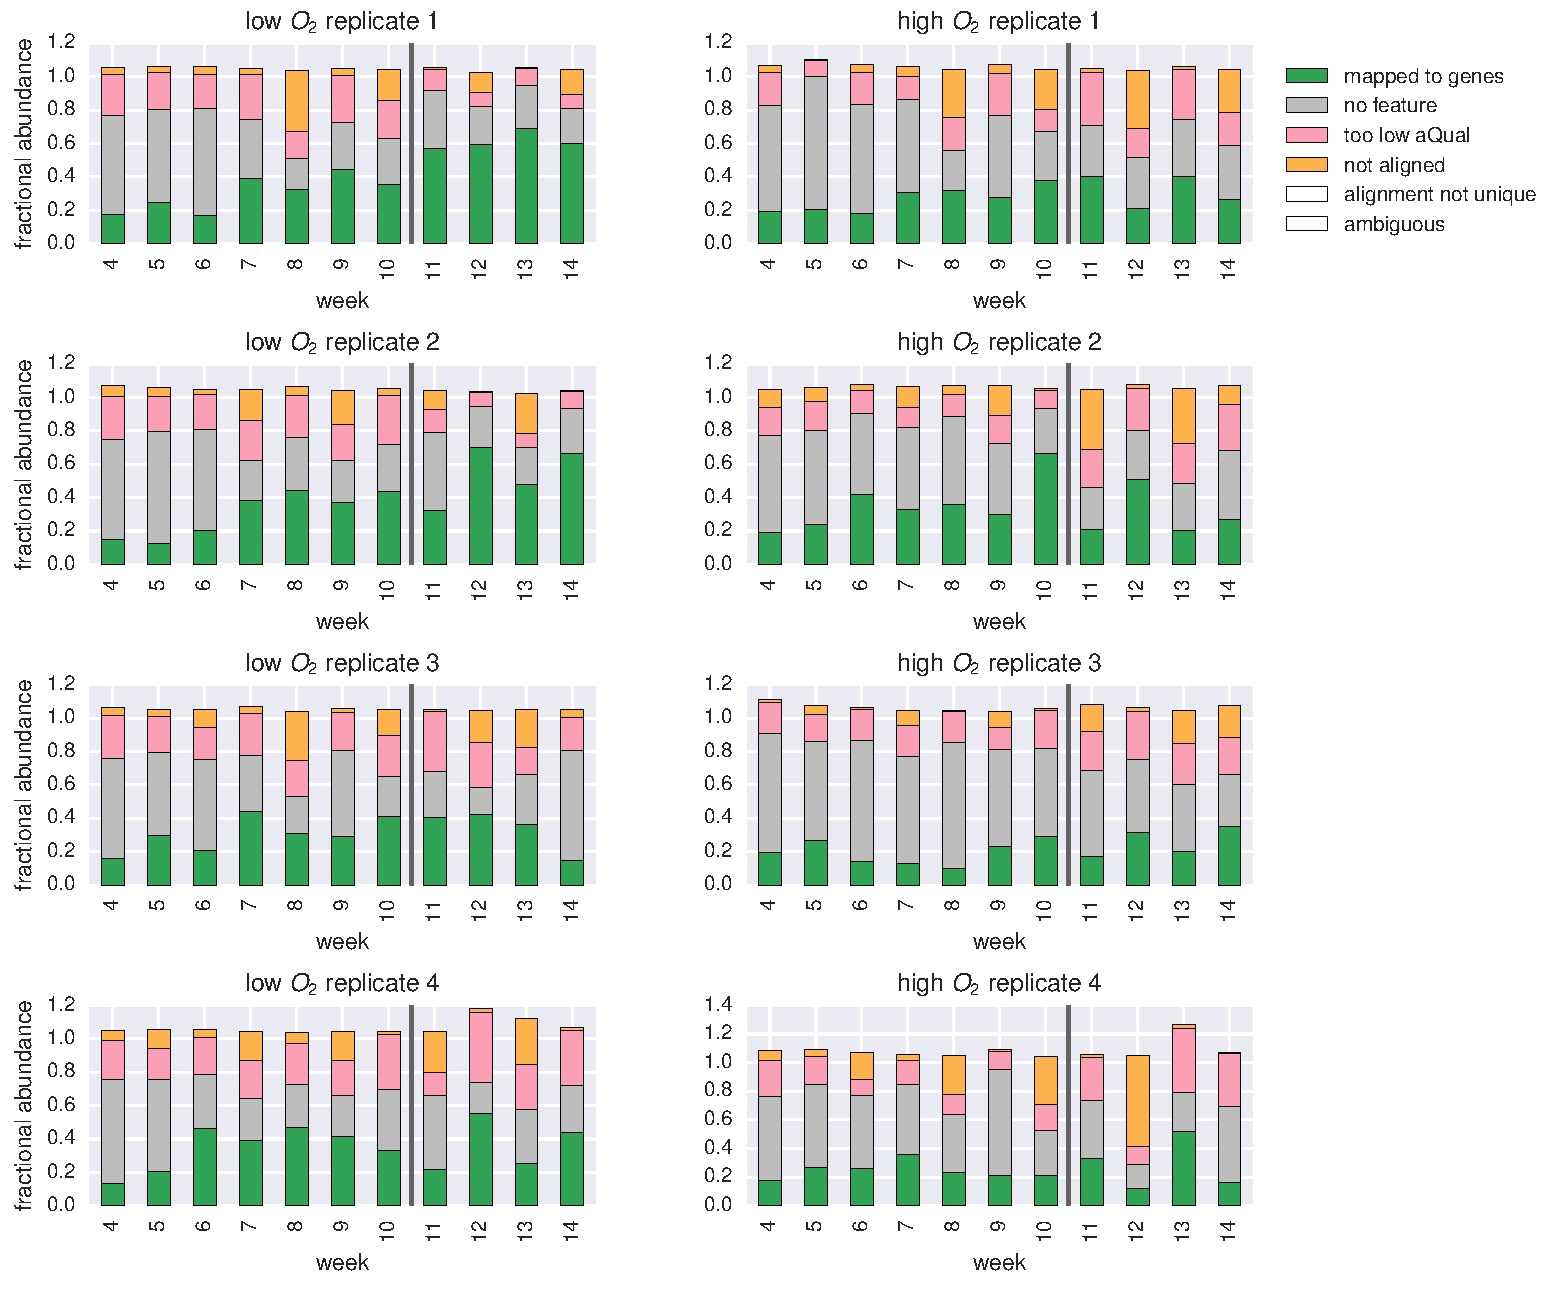
\includegraphics[width=1.0\textwidth]{./tex/chapter2/figures/170316_fracs_mapped_unmapped_etc.pdf}
    \begin{singlespace}
    \caption[Efficacy of mapping RNA-seq to MEGAHIT contigs]{
        Efficacy of mapping RNA-seq to MEGAHIT contigs.
        Bar heights are fractions of reads with respect to the original \texttt{.fastq} files.
        Bar height totals are noticeably greater than one for samples with a larger fraction of reads that map equally well to multiple loci.
        Such multiply mapped reads are included in the pink bar due to being assigned a quality score of zero by BWA-MEM.
        }
    \label{fig:rna_mapping_bars}
    \end{singlespace}
\end{figure}

\subsubsection{Highest Expressed Proteins}
% TODO: add table of highest expressed proteins, and describe.

The top genes include many methanotrophy genes, especially subunits of methane monooxygenase and methanol dehydrogenase (Table \ref{table:top_genes}).
Other highly expressed methylotrophy genes encode products including 3-hexulose-6-phosphate synthase, transketolase, formaldehyde-activating enzyme, and 3-hexulose-6-phosphate isomerase.
The presence of key methanotrophy and methylotrophy genes agrees with the Elviz portrait of methanotroph/methylotroph dominance in every sample.
Other highly expressed genes allow speculation for metabolic roles of other organisms.

Two phage proteins are near the top of the list: Capsid protein (F protein), and Microvirus H protein (pilot protein) (Figures \ref{fig:phage_protein_F}, \ref{fig:phage_pilot_protein}). %
%WTF... Group II intron-encoded protein LtrA ??  http://www.uniprot.org/uniprot/P0A3U0
Phage blooms could contribute to the apparent stochasticity in community rarefaction.
%?? Get isolate stats?? We hoped to beat the benchmark of mapping to the isolates:  median XX %.

Note that Table \ref{table:top_genes} does not include normalization for gene length or sample sequencing depth.
Before dividing by gene length, consistency of gene lengths for loci of the same gene product should be checked.
It is possible that genes encoding product of the same name could be of varying length, depending on how Prokka handles gene fragments.

\subsubsection{Expression of Genes by Locus}

Which copes are expressed, and under which conditions?
Breaking down the expression of these genes by locus and sample reveals which copies dominate.
Many of the patterns appear to be \ce{O_2}-dependent, and/or perturbed by the \ce{O_2} condition switch for the last four samples.
% TODO: figure of expression.  Include more in appendix.
% FIGURE: pmo subunit A.
For example, the patterns for which \textit{pmoC} locus is expressed in each sample appears to be correlated with the \ce{O_2} tension in each sample (Figure \ref{fig:mmo_alpha}).
Exploration of these patterns and analysis of the genes taxonomy can shed light onto how \ce{O_2} influences community composition.

\begin{figure}[H]
\centering
    % /Users/janet/Dropbox/thesis/tex/chapter2/figures/170328_loci_read_fracs_Particulate_methane_monooxygenase_alpha_subunit_precursor--portrait--cleaned.pdf
    % /Users/janet/Dropbox/meta4_bins_data_and_files/170328_locus_expression_plots/170328_loci_read_fracs_Particulate_methane_monooxygenase_alpha_subunit_precursor--portrait.pdf
    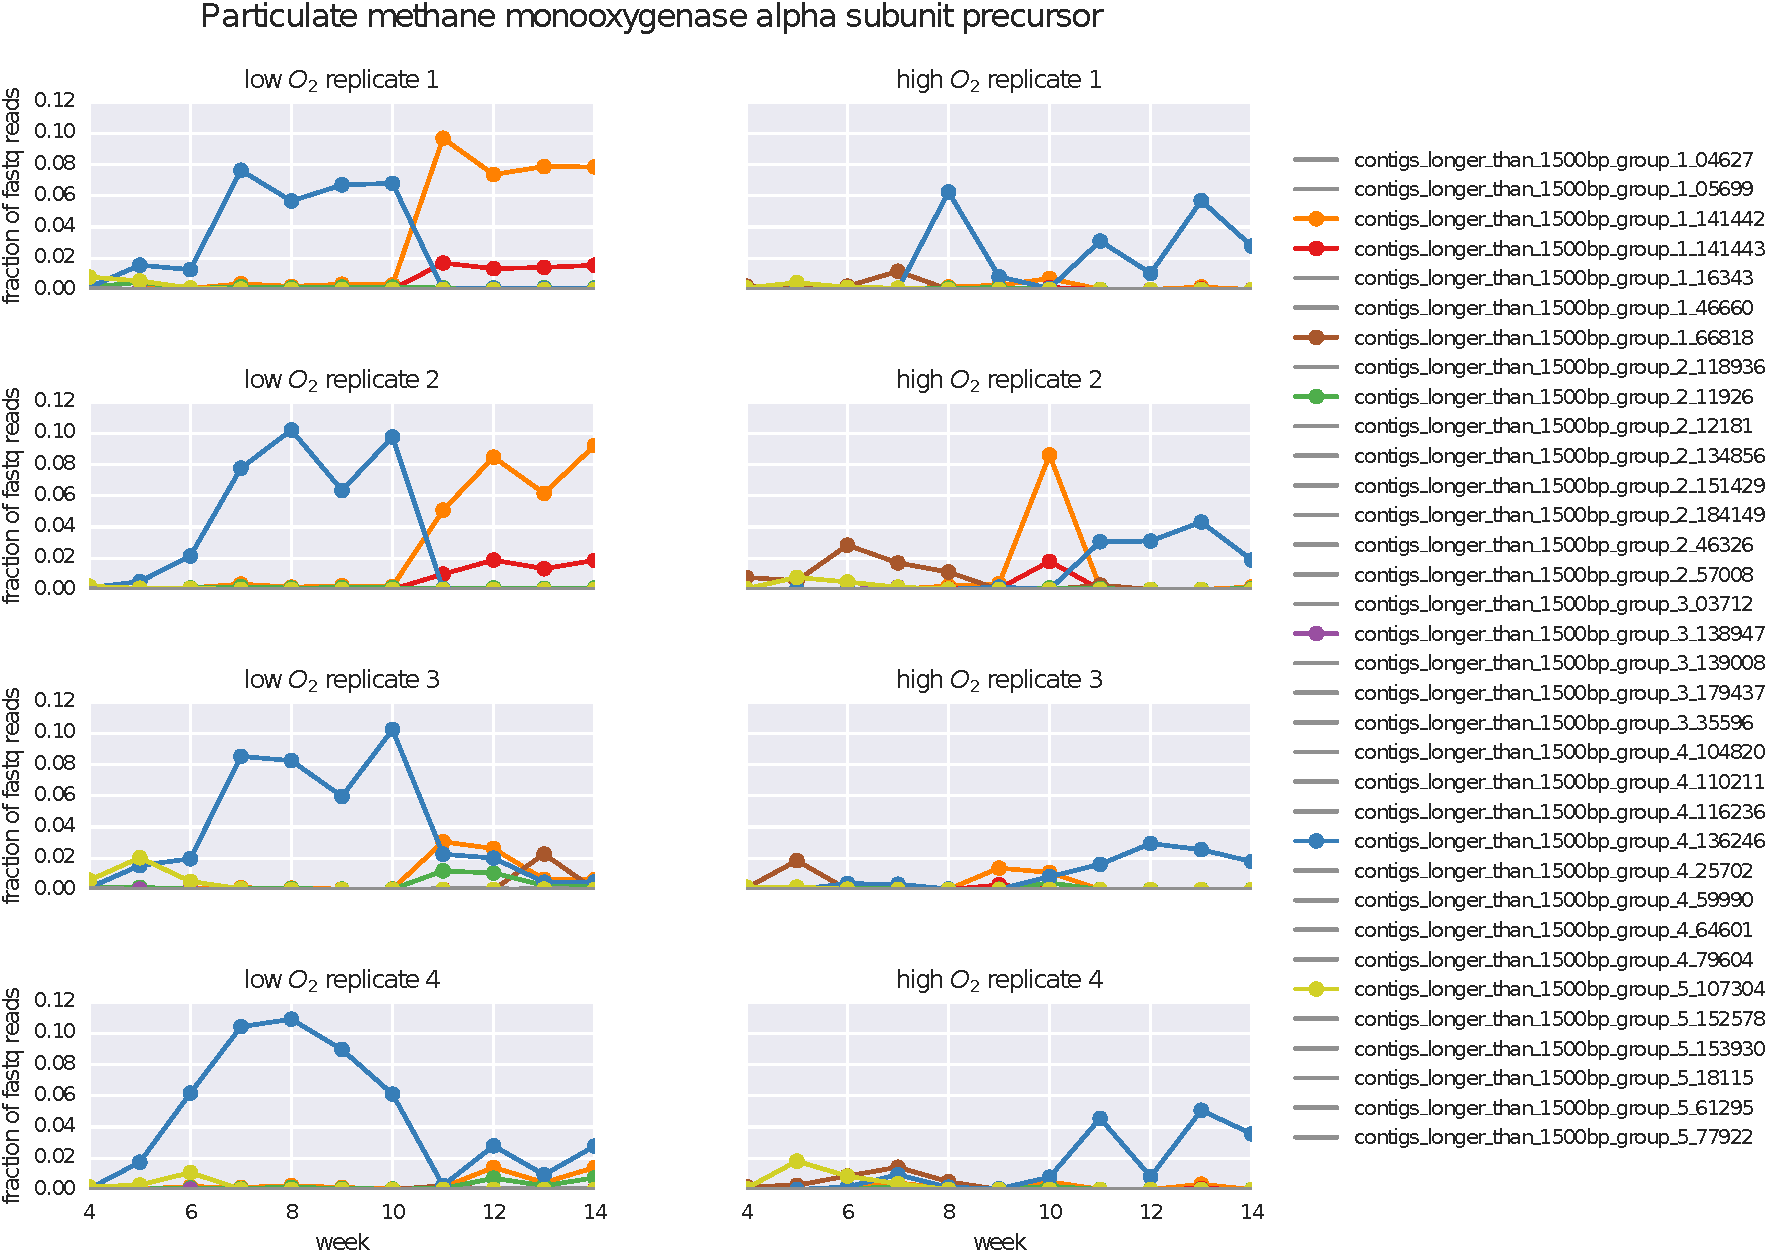
\includegraphics[width=1.0\textwidth]{./tex/chapter2/figures/170328_loci_read_fracs_Particulate_methane_monooxygenase_alpha_subunit_precursor--portrait--cleaned.pdf}
    \begin{singlespace}
    \caption[Methane monoxygenase alpha subunit locus expression profiles by sample]{
        Methane monoxygenase alpha subunit locus expression profiles by sample.
        The legend shows many genes annotated as such, but only the highest expressed loci were plotted with color.
        The gray series have nearly zero expression and thus do not rise above the x-axis.
        }
    \label{fig:mmo_alpha}
    \end{singlespace}
\end{figure}

% ----- BINNING ------
\subsection{Binning of Co-assembled Contigs}

Contigs of length $\geq$ 1.5kb were binned by MetaBAT and MyCC, two leading binning tools.
As mentioned, MyCC does not scale well to large data, so the full dataset including contigs as short as 1.5kb did not complete, even with a high performance AWS instance.

\begin{table}[H]
\centering
\begin{singlespace}
\caption[Binning results: MetaBAT \& MyCC]
	{Binning results: MetaBAT \& MyCC.}
\label{table:sample_read_sizes}
\begin{tabular}{l | cc}
 %\toprule
            & \# bins &  min contig size allowed \\  % consider fraction of contigs binned?
\midrule
	MetaBAT & 330   & 1.5kb \\
	MyCC    & 109   & 2.5kb \\
%[ec2-user@ip-10-0-0-158 metabat]$ realpath .
%/work/m4b_binning/assembly/metabat
%[ec2-user@ip-10-0-0-158 metabat]$ ls bin*.fa | wc -l
%330

%[ec2-user@ip-10-0-0-158 assembly_mycc_2.5kb_56mer_lt_0.4_st_50]$ realpath 20170131_1745_56mer_0.7_cov
%/work/m4b_binning/assembly_mycc_completed/assembly_mycc_2.5kb_56mer_lt_0.4_st_50/20170131_1745_56mer_0.7_cov
%[ec2-user@ip-10-0-0-158 assembly_mycc_2.5kb_56mer_lt_0.4_st_50]$ ls 20170131_1745_56mer_0.7_cov/Cluster*.fasta | wc -l
%109

%\bottomrule
\end{tabular}
\end{singlespace}
\end{table}

%MetaBAT suffers from low binning rates, MyCC suffers from too aggressive of binning.
Figure \ref{fig:binning_frac_reads_mapped} shows this the fraction of the metagenomes that are accounted for by the bins, as a measure of how effectively the bins describe the composition of organisms.
The two sets of lines for the MetaBAT plots measure how well the bins represent the original \texttt{.fastq} files in total (dashed lines), and how well they did using only contigs longer than 2.5kb (to better compare with the MyCC results).

\begin{figure}[H]
\centering
    % /Users/janet/Dropbox/meta4_bins_data_and_files/170201_MyCC_read_accountability_figures/170201_comparable_read_coverage_for_metabat_and_mycc_3kb.pdf
    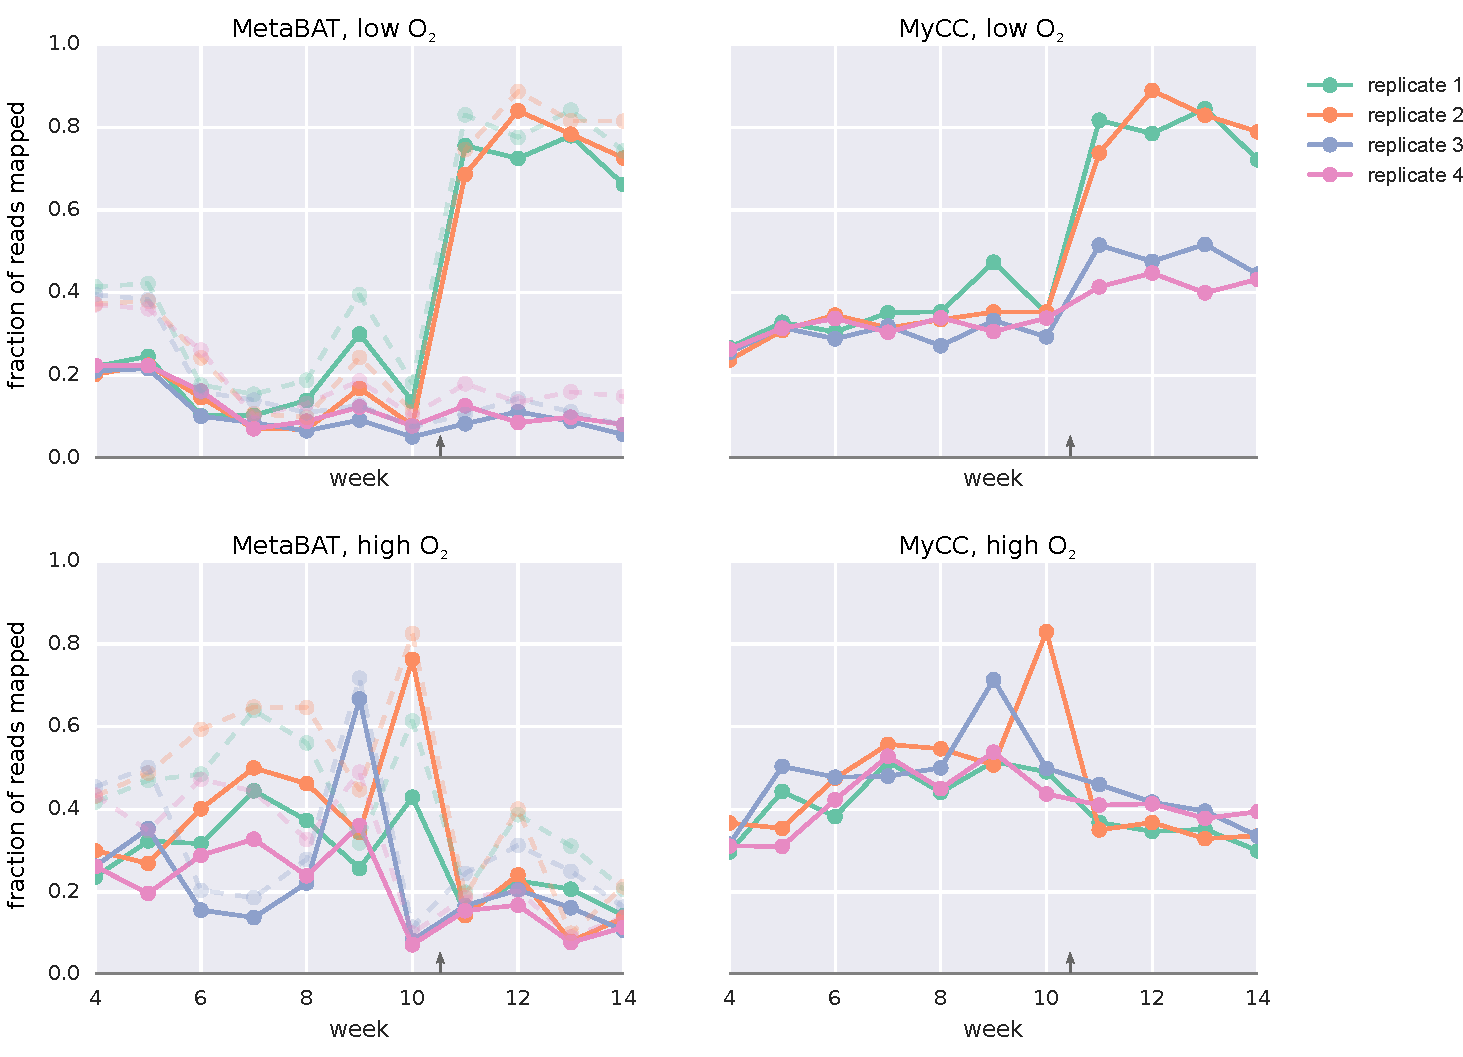
\includegraphics[width=1.0\textwidth]{./tex/chapter2/figures/170201_comparable_read_coverage_for_metabat_and_mycc_3kb--INKSCAPED.pdf}
    \begin{singlespace}
    \caption[Fraction of reads accounted for by MetaBAT and MyCC bins]{
        Fraction of reads accounted for by bins generated via MetaBAT (min contig size = 1.5kb, default settings) and MyCC (min contig size = 2.5kb, settings adjusted for memory issues).
        Points represent the fraction of reads that are associated with binned contigs for each sample.
        The solid MetaBAT lines represent the fraction of reads associated with contigs of length $\geq$ 2.5kb, as an appropriate comparison to the MyCC run.
        The dashed MetaBAT lines represent the full fraction of reads accounted for by the actual MetaBAT bins, which include contigs as short as 1.5kb.
        The arrows after week 10 in each plot indicate that all subsequent samples were treated with the opposite \ce{O_2} tension as the label indicates.
    }
    \label{fig:binning_frac_reads_mapped}
    \end{singlespace}
\end{figure}

MetaBAT with default settings produced bins with low sample accountability, whereas the MyCC bins represented a high fraction of the raw sample reads.
This represents a trade-off between precision and recall, a balance inherent to binning regardless of the tool used.

% MetaBAT comments
One striking trend in the MetaBAT results is the difference in read accountability between replicates 1/2 and 3/4 at the low \ce{O_2} state. %in the fraction of reads associated with binned contigs between low oxygen replicates 1/2 and 3/4.
The large difference is associated with the proportion of reads associated with long contigs (Supplemental Figure \ref{fig:contig_dist}).
The poorly represented samples are biased more toward short contigs.
While noting that the last 4 data points in each series have the opposite \ce{O_2} condition as the series label, see that the high \ce{O_2} samples in all four subplots are better reflected by MetaBAT bins.
This source of this conundrum has not yet been resolved, but could be due to a smear of organisms for which assembly performed poorly.
The Elviz data points towards the genus \textit{Methylobacter}, given its dominance in samples at the low-\ce{O_2} state.
BLAST or other computational tools could be used to identify the taxonomy of contigs that are not binning well. %identify the taxa for the contigs which are binning well, though high-throughput techniques would be prudent given the number of contigs.

Figure \ref{fig:mycc_binned_more_contigs} also shows that MyCC is more effective at representing the raw sequencing reads.
Upon further investigation, it was revealed that MyCC binned $>$99\% of all contigs supplied, including the shorter ($\approx$ 2.5kb) contigs which carry greater uncertainty. %(Figure \ref{fig:mycc_binned_more_contigs}).
Aggressive binning is associated with low specificity, meaning inclusion of contigs that do not belong in bins. %binning of contigs that do not belong with the others in the bin.

\begin{figure}[H]
\centering
    % /Users/janet/Dropbox/meta4_bins_data_and_files/170202_comparing_MyCC_to_metabat/170206_improved_fracs_of_contigs_binned_by_MyCC.pdf
    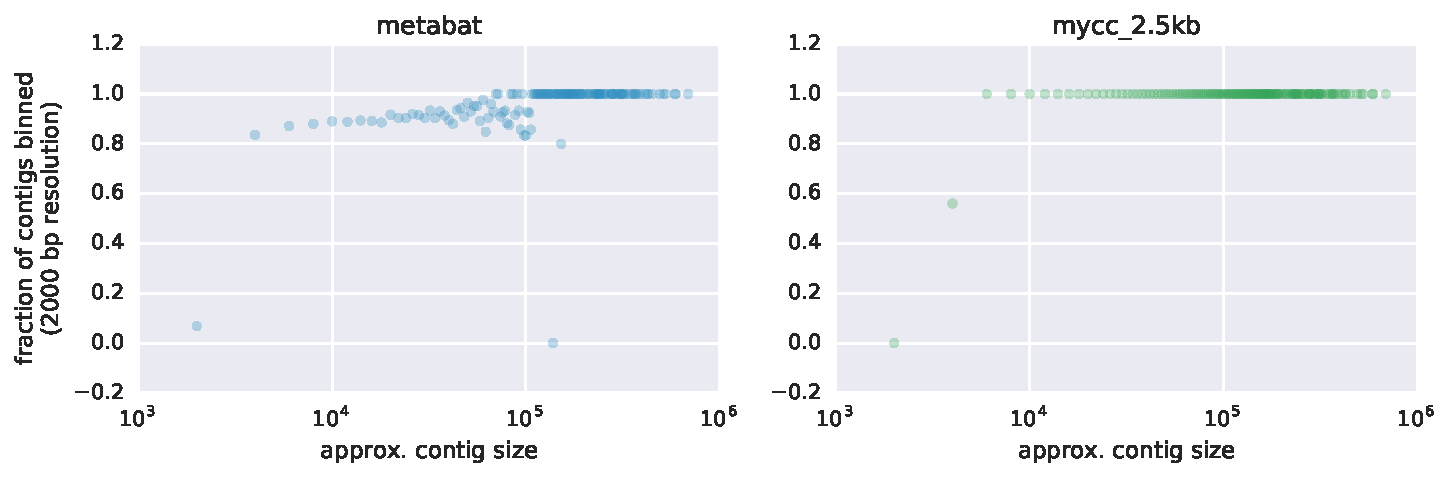
\includegraphics[width=1.0\textwidth]{./tex/chapter2/figures/170206_improved_fracs_of_contigs_binned_by_MyCC.pdf}
    \begin{singlespace}
    \caption[MyCC binned contigs more aggressively than MetaBAT]{
        MyCC binned contigs more aggressively than MetaBAT.
        With the settings used, MyCC binned $>$ 99\% of contigs at all lengths. %, for all lengths.
        The one MyCC dot near y=0.6 had a $>99\%$ binning rate as well, but is lower because the point includes contigs that were ineligible for binning (lengths below the 2.5kb cutoff).
        }
    \label{fig:mycc_binned_more_contigs}
    \end{singlespace}
\end{figure}

Figure \ref{fig:mycc_contamination} reveals the consequence of the aggressive MyCC binning: high contamination scores according to CheckM.
To test the predictive accuracy of CheckM on methylotrophic genome bins, a positive control test was used: CheckM was applied to the 55 genomes used in the isolate studies.
While the marker lineages used were often surprising (e.g. Rhizobiales, Actinomycetales), the completeness and contamination statistics CheckM returned for these positive controls were nearly perfect (Table \ref{tab:checkm_isolate}).
Thus future binning efforts should aim for nearly 100\% completeness and less than a few percent contamination, even when CheckM uses the default (non-methylotrophic) marker lineages.
High measures of strain heterogeneity may be tolerated, as some of these isolates were estimated as having 100\% strain heterogeneity  (Table \ref{tab:checkm_isolate}).
% high sensitivity, low specificity.

Given the small fraction of the metagenome reads explained by MetaBAT (Figure \ref{fig:mycc_contamination}), and high contamination scores of the MyCC bins (Figure \ref{fig:mycc_contamination}), binning has been placed on hold.
See Section \ref{chA_future_steps} below for suggested next steps in the binning workflow.


\begin{figure}[H]
\centering
    % /Users/janet/Dropbox/meta4_bins_data_and_files/170202_comparing_MyCC_to_metabat/170202_MyCC_has_higher_contamination.pdf
    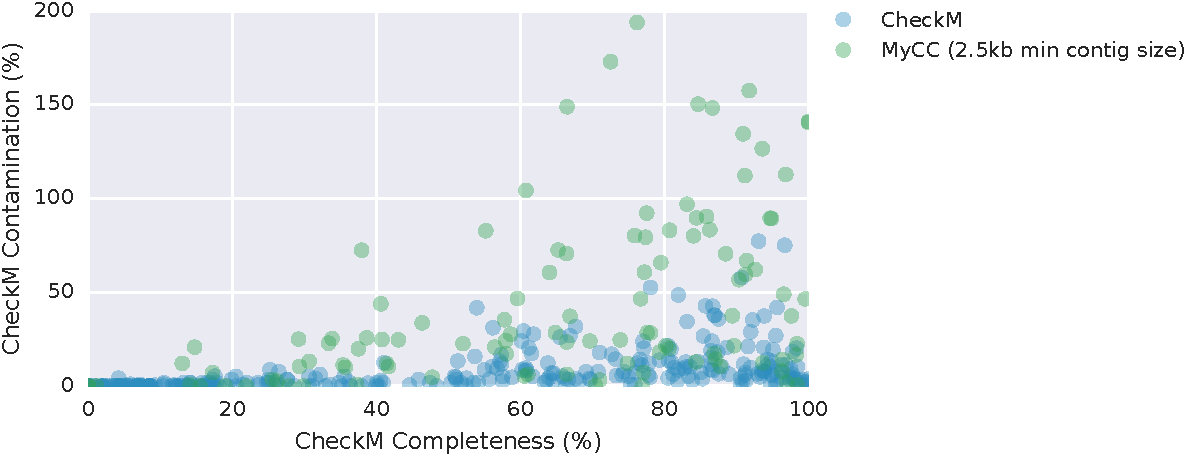
\includegraphics[width=1.0\textwidth]{./tex/chapter2/figures/170202_MyCC_has_higher_contamination--cleaned.pdf}
    \begin{singlespace}
    \caption[MyCC bins have higher contamination scores than MetaBAT bins]{
        MyCC bins have higher contamination scores than MetaBAT bins.}
    \label{fig:mycc_contamination}
    \end{singlespace}
\end{figure}

% ----- BIN TAXONOMY ------
\subsection{Bin Taxonomy}

Once final bins are in hand, taxonomic labels need to be assigned.
This can be done by aggregating information from several sources, including the CheckM marker gene set (coarse label), PhyloPhlAn results (maximally specific), and average nucleotide identity (ANI, below).

PhyloPhlAn was applied to the MetaBAT bins, producing taxonomic labels that did not agree particularly well with the CheckM labels.
This adds motivation for revisiting binning before describing the broad community composition in terms of genome bins.
% TODO: show data on this?  Put in Appendix?

% ----- ANI ------
\subsection{Average Nucleotide Identity (ANI)}

Average nucleotide identity (ANI) can also contribute evidence for taxonomic assignments, especially in cases such as this project when there are many environmental isolates from the exact ecosystem to use as references.
The JGI ANI tool was used on all pairs of MetaBAT bins and isolate genomes, producing a large matrix of ANI values, a subset of which is shown in Figure \ref{fig:ANIs}.

\begin{figure}[H]
\centering
    % /Users/janet/Dropbox/thesis/tex/chapter2/figures/170123_frac_reads_binned_at_different_contig_lengths_and_total--INKSCAPED.pdf
    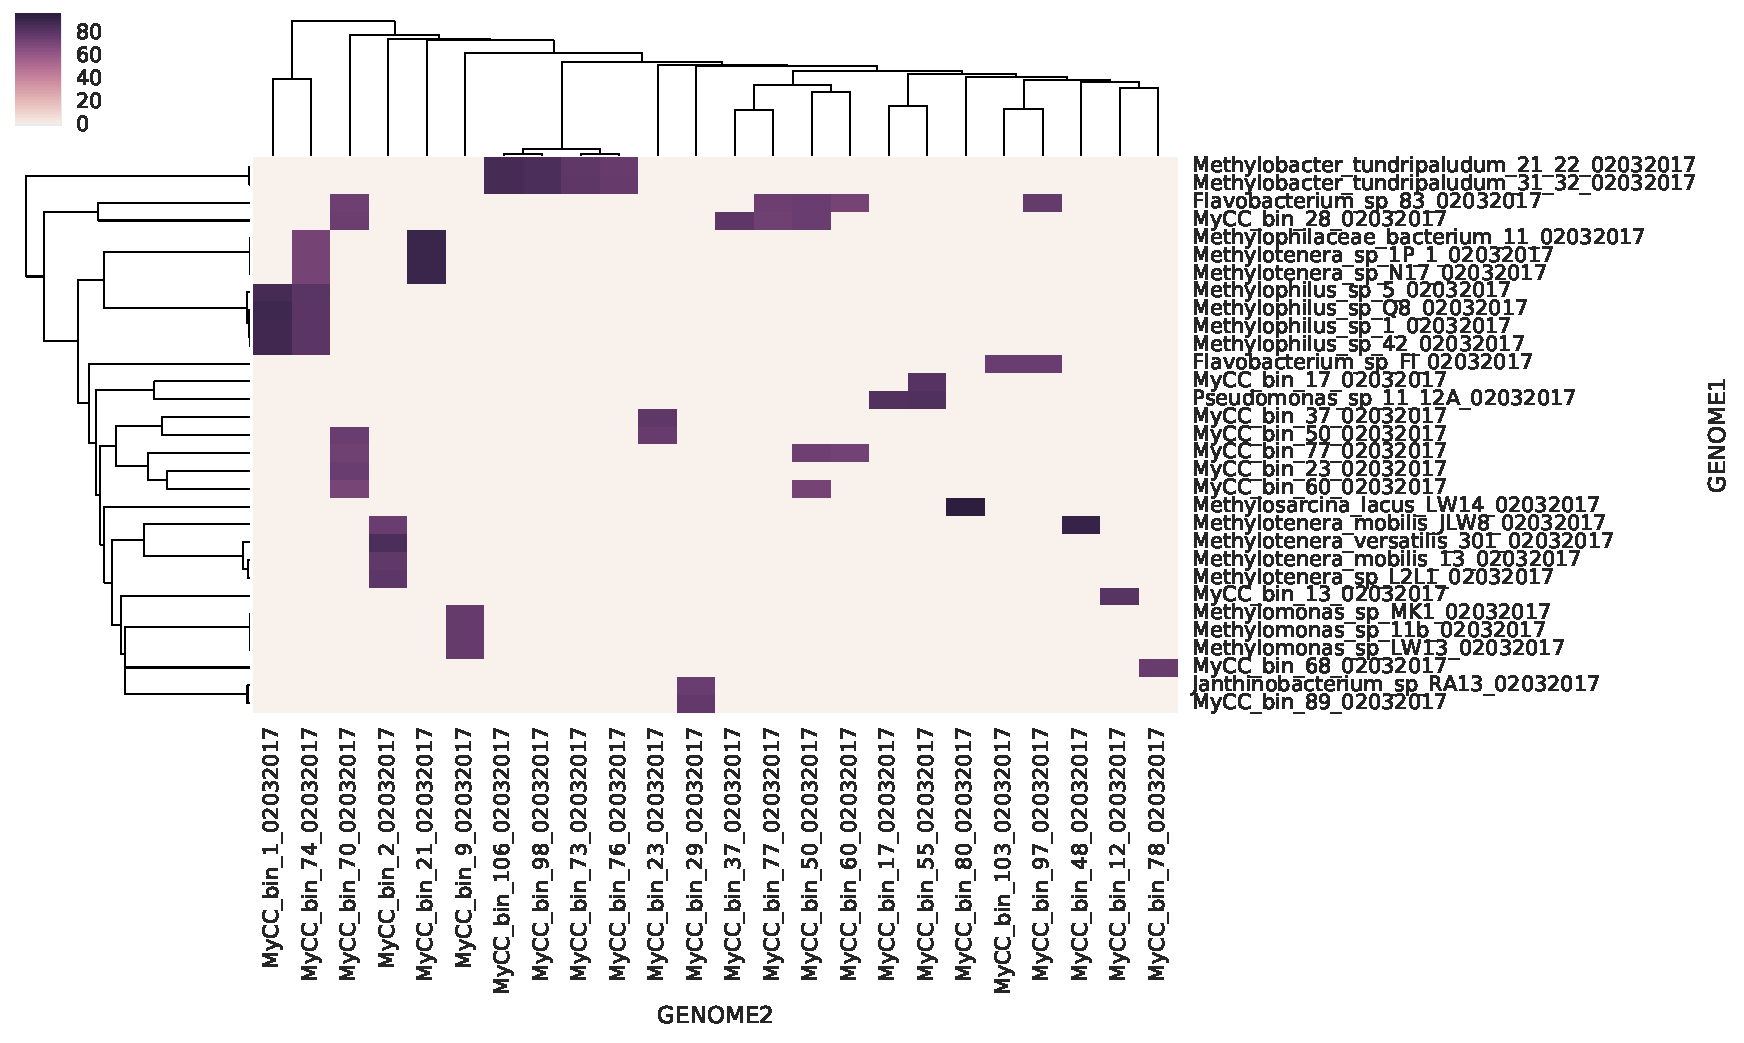
\includegraphics[width=1.0\textwidth]{./tex/chapter2/figures/170203_demo_of_ANI_heatmap.pdf}
    \begin{singlespace}
    \caption[Demo use of ANI to infer taxonomy of genome bins]{
        Demo use of ANI to infer taxonomy of genome bins.
        ANIs between all pairs of bins, and all isolate/bin pairs was computed, tabulated, and plotted to identify taxonomy of genome bins.
        This strategy, in conjunction with taxonomy calls by PhyloPhlAn \cite{segata2013} are recommended for taxonomic assignments when the final bins are identified.
        This clustermap was produced from raw ANI statistics via Seaborn (\url{https://github.com/mwaskom/seaborn}).}
    \label{fig:ANIs}
    \end{singlespace}
\end{figure}

% ------ FUTURE STEPS
\section{Future Steps}
\label{chA_future_steps}


%Big picture
This analysis aimed to describe a wholistic picture of the microbes in the mixtures, and assess how gene expression supports methane oxidation.
This thesis identified the key trends, but more precise understanding can be gained by diving deeper into many of the topics described.
Insights gained by iterating through pipeline steps have revealed possibilities to improving the analysis by modifying each step, as described in the following sections.

% ----- General NEXT STEPS ------
\subsection{Goal Setting for Future Directions}

This thesis highlights the challenge of information loss at each step of the analysis pipeline (recall the pipeline analogy in Figure \ref{fig:pipe_leaks}).
Give that the current goals are to describe broad trends of microbial abundance and activity, setting specific goals for information retention in future work is essential.
For example, substantial information in the metagenome \texttt{.fastq} files was lost along the path from raw reads to binned contigs.
Before future binning work is done, measurement of the upper-bound of binning success should be measured.
Specifically, the upper bound for the fraction of the metagenome and metatranscriptome reads that can be explained by metagenome bins can be calculated by counting all reads that align to contigs longer than 1.5kb, as was done in Figure \ref{fig:frac_elviz_mapped_to_contigs} for the Elviz Contigs.
If the fraction of reads mapping to these longer contigs is not sufficient for future publication, assembly should be re-visited (see below), or goals should be readjusted.

% TODO: insert figure of upper-bound for binning potential of these metagenomes.

% ----- Multiply Mapped Reads: NEXT STEPS ------
\subsection{Investigate Multiply Mapped Reads}
\label{sect:multiply_mapped_reads}

If the aim is to describe the community composition and gene expression broadly, investigation of multiply mapped reads is key.
As mentioned, BWA-MEM flags reads that map equally well to two loci as having a quality score of zero.
This means that any gene that appears twice in the reference contigs will have zero reads mapped to it.
Similarly, two homologous genes that attract a similar set of reads will have under-estimated gene expression.

This loss of multiply mapped reads is expected to be a problem for highly conserved genes such as particulate methane monooxygenase (pMMO).
Estimations of methanotroph abundances that rely on counting reads that map to various pMMO copies should have large associated uncertainty values.
One possible way to handle these data is to have three statistics associated with read counts for each gene.
The classically reported BWA-MEM read count will be preserved, but a second column could represent the number of additional reads that could be assigned to a gene if multiply mapped reads were spread evenly across their potential reference targets.
To give that number context, it would be beneficial to have a third column informing how many genes were similar enough to have caused read mapping ambiguity.

% ----- ASSEMBLY NEXT STEPS ------
\subsection{Assembly: Next Steps}
\label{sect:assembly_discussion}

Like all steps of metagenomics, assembly in itself is an art.
There is not one best assembly per data set, as two different research goals could lead to two different ideal assemblies.
For this thesis, the goal was a wholistic portrait of which organisms are present in natural communities.
While the assembly used throughout this chapter was appropriate for that question, there is potential to use additional assemblies to target particular organisms of interest.

%Re-assemble to find rare ones
New assemblies could be done with the aim of making contigs that bin a particular organism well.
The enumerations of the taxa present in each sample, the gene expression profiles, and trends across samples will be explored to identify uncultivated taxa to target.
For example, it is hypothesized that there is a "smear" of similar uncultivated \textit{Methylobacter} strains in these samples.
If genes thought to be associated with different \textit{Methylobacter} strains are found in particular samples, those could be re-assembled separately to get longer \textit{Methylobacter} contigs and thus better bins.
Another possibility is to iteratively bin, remove reads that map to those bins, and re-assemble the leftovers.
These approaches may also lead to bins of important non-methylotrophs, whose metabolic role is least understood.

%This is a computationally expensive and likely laborious path to wholistic community descriptions, but is possible.

% ----- BINNING NEXT STEPS ------
\subsection{Binning: Next Steps}

The analysis shown in this chapter highlights great opportunity to improve the bins and potentially allow for wholistic descriptions of the communities.
The easiest first step is to iteratively test the performance of MetaBAT with different binning parameters as the authors suggest.
The resulting bins can be assessed, again by (a) CheckM completeness and contamination scores, (b) fraction of metagenomes that are attracted to bins, and (c) the fraction of transcriptomes that are attracted to them.
Special care can be taken to bin \textit{Methylobacter} strains.

In addition, there are many tools which have not yet been tried.
One promising tool from the Banfield Lab \cite{sieber2017}\footnote{\url{http://biorxiv.org/content/early/2017/02/11/107789}} just appeared on the Biology preprint server, bioRxiv.
This tool uses an ensemble of binning algorithms (MetaBAT\cite{metabat2015}, MaxBin \cite{wu2015}, CONCOCT \cite{concoct2014} and tetraESOMs \cite{dick2009}).
It counts the number of single-copy marker genes in candidate bins, removes good looking bins, and re-bins the remaining contigs.
Given the broad efficacy of ensemble methods in machine learning, exploration of this tool is highly recommended.



% ----- BIOLOGY NEXT STEPS ------
\subsection{Biology: Next Steps}

The dataset prepared in this analysis allows investigation of many biological questions.
Many of these questions are best answered with genome bins.
For example, one topic of excitement in the field of methylotrophy pertains to two alternative methanol dehydrogenase systems.
Recently it has been discovered that some organisms prefer to use lanthanum-dependent \textit{xox} methanol dehydrogenases, rather than the classically studied \textit{mdh} methanol dehydrogenases. %TODO: cite
Though lanthanum was not intentionally supplied to the organisms in this study, it is possible that lanthanum was present in trace amounts.
Identification of expression levels of these two methanol dehydrogenase alternatives in these samples will be explored soon.

Not all questions, however, require genome bins.
Building taxonomic trees of the various signature genes such as methane monooxygenase can give higher resolution insight into community composition inferred in Figures \ref{fig:4dominant_groups}, \ref{fig:dominant_genera}.
There is also potential to explore signatures of phage in the existing contigs.


% ------ CONCLUSIONS
\section{Conclusions}

In conclusion, this 88-metagenome, 88-metatranscriptome data set was designed to allow identification of dominant taxa and gene expression in a natural methane oxidizing microbial community.
The Elviz data was aggregated on taxonomic label to illustrate the fractions of the metagenomes attributed to different taxa (see Figures \ref{fig:4dominant_groups}, \ref{fig:dominant_genera}).
These data were not appropriate for comparison across samples, or assembly into contigs, so an assembly was done with nearly all of the metagenomes.
These contigs were binned into a draft set of bins, which highlighted the challenge of getting enough good bins to illustrate the dynamics of an entire population.
% TODO: suggest quality checks so we know how good the set is.
% TODO: note dominant taxa

The contigs were annotated and the genetic content was explored.
In total, 921,431 million genes were identified, encoding 107,900 different proteins.
\ce{O_2}-dependent trends in locus expression were identified, supporting evidence that \ce{O_2} is an important and only somewhat understood factor in community composition and function.

The biology inferred in this preliminary round of studies drove new ideas for iterating through the pipeline again, with new goals and refinement strategies in mind.
While the community structure may be too complex for current binning tools to explain without extensive manual labor, targeting particular taxa for binning will allow observation of community dynamics for the major players.
In addition, the ability to extract more information about community structure and dynamics is explored in Chapter \ref{chapter:C}.


